%%%%%%%%%%%%%%%%%%%%%%%%%%%%%%%%%%%%%%%%%
% University Assignment Title Page 
% LaTeX Template
% Version 1.0 (27/12/12)
%
% This template has been downloaded from:
% http://www.LaTeXTemplates.com
%
% Original author:
% WikiBooks (http://en.wikibooks.org/wiki/LaTeX/Title_Creation)
%
% License:
% CC BY-NC-SA 3.0 (http://creativecommons.org/licenses/by-nc-sa/3.0/)
% 
% Instructions for using this template:
% This title page is capable of being compiled as is. This is not useful for 
% including it in another document. To do this, you have two options: 
%
% 1) Copy/paste everything between \begin{document} and \end{document} 
% starting at \begin{titlepage} and paste this into another LaTeX file where you 
% want your title page.
% OR
% 2) Remove everything outside the \begin{titlepage} and \end{titlepage} and 
% move this file to the same directory as the LaTeX file you wish to add it to. 
% Then add %%%%%%%%%%%%%%%%%%%%%%%%%%%%%%%%%%%%%%%%%
% University Assignment Title Page 
% LaTeX Template
% Version 1.0 (27/12/12)
%
% This template has been downloaded from:
% http://www.LaTeXTemplates.com
%
% Original author:
% WikiBooks (http://en.wikibooks.org/wiki/LaTeX/Title_Creation)
%
% License:
% CC BY-NC-SA 3.0 (http://creativecommons.org/licenses/by-nc-sa/3.0/)
% 
% Instructions for using this template:
% This title page is capable of being compiled as is. This is not useful for 
% including it in another document. To do this, you have two options: 
%
% 1) Copy/paste everything between \begin{document} and \end{document} 
% starting at \begin{titlepage} and paste this into another LaTeX file where you 
% want your title page.
% OR
% 2) Remove everything outside the \begin{titlepage} and \end{titlepage} and 
% move this file to the same directory as the LaTeX file you wish to add it to. 
% Then add %%%%%%%%%%%%%%%%%%%%%%%%%%%%%%%%%%%%%%%%%
% University Assignment Title Page 
% LaTeX Template
% Version 1.0 (27/12/12)
%
% This template has been downloaded from:
% http://www.LaTeXTemplates.com
%
% Original author:
% WikiBooks (http://en.wikibooks.org/wiki/LaTeX/Title_Creation)
%
% License:
% CC BY-NC-SA 3.0 (http://creativecommons.org/licenses/by-nc-sa/3.0/)
% 
% Instructions for using this template:
% This title page is capable of being compiled as is. This is not useful for 
% including it in another document. To do this, you have two options: 
%
% 1) Copy/paste everything between \begin{document} and \end{document} 
% starting at \begin{titlepage} and paste this into another LaTeX file where you 
% want your title page.
% OR
% 2) Remove everything outside the \begin{titlepage} and \end{titlepage} and 
% move this file to the same directory as the LaTeX file you wish to add it to. 
% Then add %%%%%%%%%%%%%%%%%%%%%%%%%%%%%%%%%%%%%%%%%
% University Assignment Title Page 
% LaTeX Template
% Version 1.0 (27/12/12)
%
% This template has been downloaded from:
% http://www.LaTeXTemplates.com
%
% Original author:
% WikiBooks (http://en.wikibooks.org/wiki/LaTeX/Title_Creation)
%
% License:
% CC BY-NC-SA 3.0 (http://creativecommons.org/licenses/by-nc-sa/3.0/)
% 
% Instructions for using this template:
% This title page is capable of being compiled as is. This is not useful for 
% including it in another document. To do this, you have two options: 
%
% 1) Copy/paste everything between \begin{document} and \end{document} 
% starting at \begin{titlepage} and paste this into another LaTeX file where you 
% want your title page.
% OR
% 2) Remove everything outside the \begin{titlepage} and \end{titlepage} and 
% move this file to the same directory as the LaTeX file you wish to add it to. 
% Then add \input{./title_page_1.tex} to your LaTeX file where you want your
% title page.
%t
%%%%%%%%%%%%%%%%%%%%%%%%%%%%%%%%%%%%%%%%%
\title{Chatbot hỗ trợ thương mại điện tử}
%----------------------------------------------------------------------------------------
%	PACKAGES AND OTHER DOCUMENT CONFIGURATIONS
%----------------------------------------------------------------------------------------

\documentclass[12pt]{article}
\usepackage[T5]{fontenc}
\usepackage[utf8]{inputenc}
%\usepackage[utf8]{vietnam}
\usepackage{indentfirst} % thục dòng cái dòng đầu tiên 
\usepackage[vietnamese,english]{babel}
\usepackage{amsmath}
\usepackage{graphicx}
\usepackage[colorinlistoftodos]{todonotes}
\usepackage{listings}
\usepackage{xcolor}
\lstset{basicstyle=\ttfamily,
  showstringspaces=false,
%   commentstyle=\color{red},
%   keywordstyle=\color{blue}
}
\usepackage{hyperref}
\hypersetup{
    colorlinks=true,
    linkcolor=blue,
    filecolor=magenta,      
    urlcolor=cyan,
}


\renewcommand{\lstlistingname}{Mã }% Listing -> Algorithm
\addto\captionsenglish{\renewcommand{\figurename}{Hình}}

\begin{document}

\begin{titlepage}

\newcommand{\HRule}{\rule{\linewidth}{0.5mm}} % Defines a new command for the horizontal lines, change thickness here

\center % Center everything on the page
 
%----------------------------------------------------------------------------------------
%	HEADING SECTIONS
%----------------------------------------------------------------------------------------

\textsc{\LARGE Đại học Khoa học tự nhiên}\\[1.5cm] % Name of your university/college
\textsc{\Large Ngành hệ thống thông tin}\\[0.5cm] % Major heading such as course name
\textsc{\large Môn học: HỆ CƠ SỞ DỮ LIỆU NÂNG CAO }\\[0.5cm] % Minor heading such as course title

%----------------------------------------------------------------------------------------
%	TITLE SECTION
%----------------------------------------------------------------------------------------

\HRule \\[0.4cm]
{ \huge \bfseries 
Chatbot hỗ trợ thương mại điện tử
}\\[0.4cm] % Title of your document
\HRule \\[1.5cm]
 
%----------------------------------------------------------------------------------------
%	AUTHOR SECTION
%----------------------------------------------------------------------------------------

\begin{minipage}{0.5 \textwidth}
\begin{flushleft} \large
\emph{Học viên:}\\
Thái Thiện 17C12031 \\ % Your name
Lê Võ Minh Thư 17C12033
\end{flushleft}
\end{minipage}
~
\begin{minipage}{0.45 \textwidth}
\begin{flushright} \large
\emph{Giảng viên:} \\
TS. Nguyễn Trần Minh Thư % Supervisor's Name
\end{flushright}
\end{minipage}\\[1cm]

% If you don't want a supervisor, uncomment the two lines below and remove the section above
%\Large \emph{Author:}\\
%John \textsc{Smith}\\[3cm] % Your name

%----------------------------------------------------------------------------------------
%	DATE SECTION
%----------------------------------------------------------------------------------------

% I don't want day because it is English
% {\large \today}\\[2cm] % Date, change the \today to a set date if you want to be precise

%----------------------------------------------------------------------------------------
%	LOGO SECTION
%----------------------------------------------------------------------------------------


\includegraphics{logo/rsz_3logo-khtn.png}\\[1cm] % Include a department/university logo - this will require the graphicx package
 
%----------------------------------------------------------------------------------------

\vfill % Fill the rest of the page with whitespace

\end{titlepage}

\tableofcontents
\newpage

\section{Bài toán đặt ra}

\subsection{Chatbot}
	Chatbot là một hệ thống tự động có thể giao tiếp với người dùng để thực hiện các thao tác được lập trình sẵn.  Trong thương mại điện tử, Chatbot được dùng thay nhân viên trực tổng đài để tiếp khách hàng và giúp đỡ khách hàng một số tác vụ đơn giản như tìm kiếm sản phẩm. Từ đó giúp tiết kiệm nhân công, kênh liên lạc luôn thông suốt.
	

\subsection{Thông tin ứng dụng}

Trong đồ án này, nhóm chúng tôi xây dựng một chatbot cho trang thương mại điện tử "Xưởng may Thiên Phúc\footnote{\url{http://xuongmaythienphuc.vn/}}". Chatbot sẽ có tính năng chính là tìm kiếm và hiển thị thông tin sản phẩm. Mỗi sản phẩm trả về sẽ kèm đường dẫn tới trang thương mại điện tử, giúp khách hàng dễ dàng đăt hàng.


%%%%%%%%%%%%%%%%%%%%%START EXAMPLE THING%%%%%%%%%%%%%%%
% % % Commands to include a figure:
% \begin{figure}[h]
% \centering
% 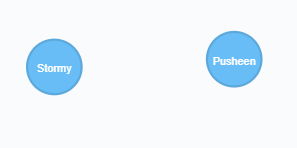
\includegraphics[width=0.5\textwidth]{image/node.PNG}
% \caption{\label{fig:node} Nút}
% \end{figure}


% % chuong 3
% \section{Chèn đoạn code}


% ví dụ code \ref{lst:vdcode} là code python 


% \begin{lstlisting}[caption={Đoạn code}, label={lst:vdcode}, language=python]
% s = "I am Pusheen the cat"
% print(s)
% \end{lstlisting}

% ví dụ trích dẫn \cite{robinson2013graph}
%%%%%%%%%%%%%% END EXAMPLE THING %%%%%%%%%%%%%%%%%%%%%%%%%

\section{Xây dựng ứng dụng}

\subsection{Mô hình hóa dữ liệu}

Dữ liệu nhập vào sẽ có dạng bảng có nhiều cột. Nhưng ta chỉ cần quan tâm 4 cột: Nhóm hàng, Mã hàng, Tên hàng, Giá bán. Dữ liệu cần nhập vào có bảng như dưới đây.

\begin{center}
 \begin{tabular}{||c c c c||} 
 \hline
 Nhóm hàng & Mã hàng & Tên hàng & Giá bán \\ [0.5ex] 
 \hline\hline
 Đồ Bộ Nữ & 1675NgoiXLSale & Set Bộ Dài Cam Ngói Phối Màu Sành Điệu & 120000 \\ 
 \hline
 Đầm dự tiệc & 1628DoXXLSale & Đầm đỏ body dự tiệc phối ren đuôi cá & 155000 \\
 \hline
  Đầm dự tiệc & 1573LSale & Đầm form chữ A tay ren cổ kết pha lê  & 120000 \\ [1ex] 
 \hline
\end{tabular}
\end{center}

Dữ liệu trong Neo4j sẽ có 4 thực thể: \pagebreak

\textbf{PRODUCT} : Sản phẩm 
\begin{itemize}
\item name (String) : Tên sản phẩm, lấy trực tiếp từ cột Tên Hàng trong bảng nguồn. 
\item normalized\_name (String) : Tên sản phẩm sau khi chuẩn hóa bằng cách bỏ dấu tiếng Việt và đổi sang viết thường. Chuẩn hóa giúp truy vấn tiếng Việt không dấu. 
\item url (String) : Đường dẫn tới sản phẩm trên trang "Xưởng may Thiên Phúc" 
\end{itemize}


\textbf{CATEGORY} : Nhóm hàng 
\begin{itemize}
\item name (String) : Tên nhóm hàng, lấy trực tiếp từ cột Nhóm hàng trong bảng nguồn
\item normalized\_name (String) : Tên nhóm hàng sau khi chuẩn hóa bằng cách bỏ dấu tiếng Việt và đổi sang viết thường. Chuẩn hóa giúp truy vấn tiếng Việt không dấu. 
\end{itemize}

\textbf{ITEM} : Mặt hàng. 
\begin{itemize}
\item code (String) : Mã hàng trong bảng nguồn. 
\item price (int) : giá tiền (đơn vị VND)  
\end{itemize}

Quan hệ giữa các thực thể 
\begin{itemize}
\item Một PRODUCT có từ 1 đến n quan hệ BELONG\_TO với CATEGORY
\item Một CATEGORY có từ 1 đến n quan hệ BELONG\_TO với PRODUCT
\item Một PRODUCT có từ 1 đến n quan hệ HAS với ITEM 
\item Một ITEM chỉ có 1 quan hệ HAS đến 1 PRODUCT 
\end{itemize}

Có thể diễn đạt bằng lời thế này: Mỗi sản phẩm thuộc nhiều nhóm hàng và có nhiều mặt hàng. Mội mặt hàng chỉ thuộc về một sản phẩm. 

Hình \ref{fig:datastructure} biểu diễn mối quan hệ giữa các thực thể. Hình \ref{fig:datastructureexample} biểu diễn trực quan hóa trên Neo4j gồm một CATEGORY (Nhóm hàng) với 2 PRODUCT (Sản phẩm) và các ITEM (mặt hàng) của mỗi sản phẩm.  

Chiều của quan hệ không ảnh hưởng đến quá trình nạp dữ liệu và truy vấn dữ liệu trong trường hợp sử dụng của đồ án này. 

% Commands to include a figure:
\begin{figure}[h]
\centering
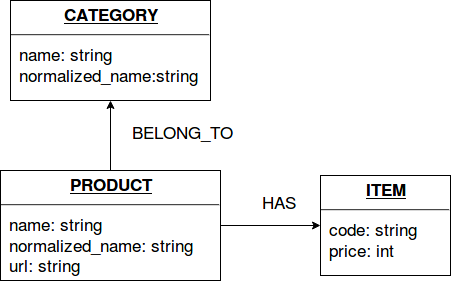
\includegraphics[width=0.5\textwidth]{image/neo4jdatastructure.png}
\caption{\label{fig:datastructure} Sơ đồ đồ quan hệ các thực thể}
\end{figure}


\begin{figure}[h]
\centering
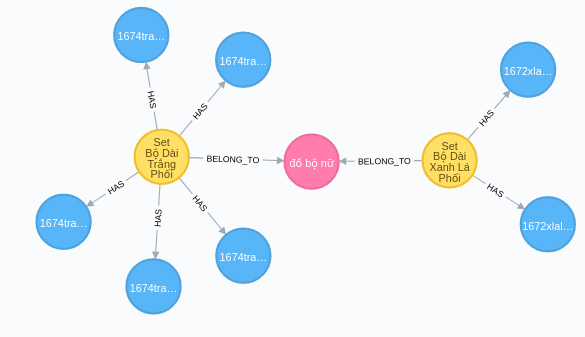
\includegraphics[width=0.5\textwidth]{imagev2/vddatamodel.png}
\caption{\label{fig:datastructureexample} Ví dụ đơn giản}
\end{figure}


\subsection{Chuyển đổi và nạp dữ liệu}
Chúng tôi chuyển đổi dữ liệu từ dạng bản sang các Neo4j Cypher, và dùng cypher đó để nạp vào cơ sở dữ liệu. Mã nguồn nằm trong thư mục csdlnc-util và hướng dẫn sử dụng được trình bày ở mục \ref{sec:csdlncutil}. Mỗi dòng trong bảng nguồn sẽ tạo ra 5 truy vấn. 

Các bước chuyển đổi: 
\begin{itemize}
\item Tạo CATEGORY 
\item Tạo PRODUCT 
\item Tạo ITEM
\item Tạo quan hệ BELONG\_TO giữa CATEGORY và PRODUCT 
\item Tạo quan hệ HAS giữa PRODUCT và ITEM
\end{itemize}

Ta lấy ví dụ, để nạp dòng đầu tiên vào Neo4j cần 5 truy vấn sau

\subsubsection{Tạo CATEGORY}\label{sec:mergecategory}
MERGE (category:CATEGORY{name: 'đồ bộ nữ', normalized\_name: 'do bo nu' })

Từ khóa MERGE sẽ tìm trong cơ sở dữ liệu thực thể CATEGORY như định nghĩa trong ngoặc tròn. Nếu không tìm được thực thể CATEGORY nào như định nghĩa, Neo4j sẽ tạo thực thể mới. Dùng MERGE thay CREATE sẽ giúp xử lý trường hợp trùng, lập nút. Ngoài ra, ở bước nạp dữ liệu, ta không cần xử lý query để xem Neo4j đã tồn tại thực thể đó chưa 

\subsubsection{Tạo PRODUCT}\label{sec:mergeproduct}

MERGE (product:PRODUCT{ name:'Set Bộ Dài Cam Ngói Phối Màu Sành Điệu', url: 'http://xuongmaythienphuc.vn/component/products/set-bo-dai-cam-ngoi-phoi-mau-sanh-dieu.html', normalized\_name: 'set bo dai cam ngoi phoi mau sanh dieu'})

\subsubsection{Tạo ITEM}\label{sec:mergeitem}

MERGE (item:ITEM{code:'1675ngoixlsale', price: 120000})

\subsubsection{Tạo mối quan hệ}\label{sec:mergerel}

\textit{Câu truy vấn tạo quan hệ BELONG\_TO:} 

\medskip

MATCH (category:CATEGORY), (product:PRODUCT) 

WHERE category.name = 'đồ bộ nữ' AND product.name = 'Set Bộ Dài Cam Ngói Phối Màu Sành Điệu'

MERGE (category)<-[:BELONG\_TO]-(product)

\bigskip

\textit{Câu truy vấn tạo quan hệ HAS:}

\medskip

MATCH (product:PRODUCT),(item:ITEM) 

WHERE  product.name = 'Set Bộ Dài Cam Ngói Phối Màu Sành Điệu' AND item.code = '1675ngoixlsale' 

MERGE (product)-[:HAS]->(item)

\bigskip

Một câu truy vấn có thể viết nhiều dòng. Nhưng mỗi dòng chỉ có thể chứa tối đa một câu truy vấn. Ta có thể nhập câu truy vấn nhiều dòng vào Neo4j Browser (Shift+Enter để xuống dòng, Ctrl + Enter để thực hiện truy vấn). Đối với các Neo4j driver, mỗi câu truy vấn là một chuỗi string có thể chứa dấu xuống hàng. Truy vấn nhiều hàng sau khi gộp lại một hàng có cùng ý nghĩa. 

\subsubsection{Gộp 5 câu truy vấn lại một câu truy vấn}
Có thể gộp cả 5 câu truy vấn trên thành 1 câu truy vấn duy nhất. Tuy nhiên, chúng tôi chưa áp dụng vào đồ án vì để giữ cho các câu truy vấn đơn giản, giúp dễ dàng gỡ lỗi khi cần thiết. Dưới đây là phương pháp gộp câu truy vấn. Phương pháp: 

\begin{itemize}
\item gộp 3 câu truy vấn MERGE tạo CATEGORY, PRODUCT, ITEM ở bước \ref{sec:mergecategory}, \ref{sec:mergeproduct}, \ref{sec:mergeitem}. 
\item bỏ vế MATCH và WHERE ở bước tạo quan hệ \ref{sec:mergerel}. 
\item gộp cả 5 MERGE lại (giữ nguyên thứ tự) thành câu truy vấn duy nhất 
\end{itemize} 

Ví dụ, trường hợp 5 câu truy vấn trên sẽ được gộp lại như sau

\medskip

MERGE (category:CATEGORY{name: 'đồ bộ nữ', normalized\_name: 'do bo nu' })

MERGE (product:PRODUCT{ name:'Set Bộ Dài Cam Ngói Phối Màu Sành Điệu', url: 'http://xuongmaythienphuc.vn/component/products/set-bo-dai-cam-ngoi-phoi-mau-sanh-dieu.html', normalized\_name: 'set bo dai cam ngoi phoi mau sanh dieu'})

MERGE (item:ITEM{code:'1675ngoixlsale', price: 120000})

MERGE (category)<-[:BELONG\_TO]-(product)

MERGE (product)-[:HAS]->(item)

\medskip

Giải thích: 3 vế MERGE đầu tiên không phụ thuộc vào định danh nào. Câu truy vấn tạo quan hệ phụ thuộc vào các định danh product, category, item. Khi đứng 1 mình, ta phải định nghĩa cho các định danh ấy bằng vế MATCH và WHERE. Tuy nhiên, khi gộp chung với các vế MERGE thì ta có thể tái sử dụng các định danh đã được định nghĩa ở các vế MERGE trên. Vì vậy, có thể bỏ các vế MATCH và WHERE. 

\bigskip

Sau khi chạy cả 5 truy vấn, hoặc một truy vấn gộp, ta đều được một đồ thị như hình \ref{fig:cypher} 

\begin{figure}[h]
\centering
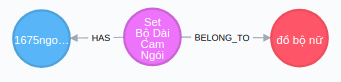
\includegraphics[width=0.5\textwidth]{imagev2/merge5cypher.png}
\caption{\label{fig:cypher} Đồ thị tạo ra từ dòng đầu tiên trong bảng nguồn}
\end{figure}

\subsection{Chatbot nền tảng Telegram}

Chatbot sẽ làm 2 việc sau: 

\begin{itemize}
\item Chuyển đổi đoạn chat của người dùng thành câu truy vấn 
\item Thực hiện truy vấn để lấy kết quả 
\item Xây dựng kết quả truy vấn thành câu trả lời cho người dùng 
\end{itemize}

Chatbot sẽ tiếp nhận yêu cầu của người dùng dưới dạng cú pháp bắt đầu bằng dấu gạch xiên "/". Khi đoạn chat không bắt đầu bằng dấu gạch xien "/" thì chatbot tự hiểu là tìm sản phẩm có tên là đoạn chat 

\subsubsection{/help} 
Hiển thị bản trợ giúp, bao gồm thông tin các câu lệnh

\subsubsection{/liet\_ke\_loai}
Liệt kê danh sách tất cả các nhóm hàng 

\subsubsection{/tim\_san\_pham <tên sản phẩm>}
Thực hiện tìm sản phẩm theo tên. Tên có thể viết có dấu hoặc không có dấu tiếng Việt. 
Câu truy vấn mẫu cho sản phẩm áo thun ("/tim\_san\_pham áo thun" hoặc "áo thun") như sau: 

\smallskip

MATCH (p:PRODUCT)-[:HAS]-(i:ITEM) 

WHERE p.name=~ '(?i).*áo thun.*' OR p.normalized\_name=~ '.*(?i)ao thun.*' 

RETURN p, i LIMIT 15

\smallskip

Ở về WHERE, dấu =~ sẽ kiểm tra các điều kiện thỏa Regular Expression (Regex) ghi trong dấu ngoặc kép. 
.*(?i)áo thun.* sẽ thỏa những câu có tồn tại từ "áo thun" (không phân biệt viết hoa, thường) trong cong. Vì vậy, vế WHERE này sẽ tìm những trường hợp mà nút PRODUCT có tên (hoặc tên không dấu) thỏa điều kiện của Regex  

Câu truy vấn trả về thông tin sản phẩm và mặt hàng 

\subsubsection{/tim\_loai <loại hoặc nhóm hàng> }

Tìm sản phẩm theo nhóm hàng.

Ví dụ: "/tim\_loai áo" sẽ tạo ra câu truy vấn sau
 
MATCH (c:CATEGORY)-[:BELONG\_TO]-(p:PRODUCT)

WHERE c.name=~'.*(?i)áo.*' OR c.normalized\_name=~'.*(?i)ao.*'  

return c, p

LIMIT 25

\smallskip

\subsubsection{/tim\_re\_hon <giá> và /tim\_mac\_hon <giá>}

Khi tìm sản phẩm theo giá, bot sẽ trả về sản phẩm gần với giá đó nhất, tùy theo người dùng muốn tìm rẻ hơn hay mắc hơn 

Ví dụ: truy vấn này tìm sản phẩm rẻ hơn 300 000 VND. Vế ORDER BY cùng từ khóa DESC sẽ xếp kết quả theo giá tiền từ cao đến thấp. Vì vậy, ta sẽ được sản phẩm gần với giá tiền ta tìm ở trên. 

MATCH (p:PRODUCT)-[:HAS]-(i:ITEM)

WHERE i.price <= 300000 

RETURN p, i 

ORDER BY i.price DESC 

LIMIT 15

\smallskip

Tương tự, bên dưới đây là ví dụ truy vấn của tìm sản phẩm mắc hơn 300000 VND. Trả về sẽ là các sản phẩm có mặt hàng có giá được xếp theo thứ tự từ 300 000 vnd trở lên. 

MATCH (p:PRODUCT)-[:HAS]-(i:ITEM)

WHERE i.price >= 300000 

RETURN p, i 

ORDER BY i.price  

LIMIT 15

\smallskip

\subsubsection{/re\_nhat và /mac\_nhat }

Trong 2 câu lệnh này, ta có thể thêm tên sản phẩm để lọc những sản phẩm có hoặc để trống tện sản phẩm để tìm với tất cả sản phẩm. 

"/re\_nhat" có câu truy vấn như sau: 

MATCH (p:PRODUCT)-[:HAS]-(i:ITEM)

return p, i 

ORDER BY i.price  

LIMIT 10

\smallskip

Dưới đây là truy vấn của "/mac\_nhat" 

MATCH (p:PRODUCT)-[:HAS]-(i:ITEM)

return p, i 

ORDER BY i.price DESC 

LIMIT 10

\smallskip

Nếu ta thêm vào tên sản phẩm, thì 2 truy vấn trên sẽ thêm vào vế WHERE để lọc kết quả theo tên sản phẩm. Dưới đây là ví dụ của truy vấn "/re\_nhat áo" 

MATCH (p:PRODUCT)-[:HAS]-(i:ITEM)

WHERE p.name=~ '.*(?i)áo.*' OR p.normalized\_name=~ '.*(?i)ao.*' 

RETURN p, i 

ORDER BY i.price  

LIMIT 10

\smallskip

Và "/mac\_nhat áo"

MATCH (p:PRODUCT)-[:HAS]-(i:ITEM)

WHERE p.name=~ '.*(?i)áo.*' OR p.normalized\_name=~ '.*(?i)ao.*' 

RETURN p, i 

ORDER BY i.price DESC 

LIMIT 10

\subsubsection{/tim\_khoang\_gia <chặn dưới> <chặn trên>}

Tìm khoảng giá sẽ trả về danh sách các sản phẩm có mặt hàng nằm trong khoảng giá đề ra. Ví dụ khi người dùng gửi tin nhắn "/tim\_khoang\_gia 200000 300000", bot sẽ tạo ra câu truy vấn sau 

MATCH (p:PRODUCT)-[:HAS]-(i:ITEM)  

WHERE i.price >= 200000 AND i.price <= 300000 

RETURN p, i 

ORDER BY i.price  

LIMIT 15

\subsubsection{/cung\_loai <mã sản phẩm>}

Chức năng này sẽ tìm sản phẩm cùng loại với sản phẩm mình đang quan tâm. Tin nhắn "/cung\_loai 816f" sẽ trả về các sản phẩm cùng loại với mặt hàng có mã 816f. Câu truy vấn được tạo ra như sau: 

MATCH (i:ITEM)-[:HAS]-(pp:PRODUCT)-[:BELONG\_TO]-(c:CATEGORY),

(c)-[:BELONG\_TO]-(p:PRODUCT)  

WHERE i.code = '816f'

RETURN p LIMIT 25



\subsubsection{Cách thức hiển thị kết quả từ câu truy vấn}

Truy vấn của câu lệnh /tim\_loai, /cung\_loai, sẽ trả chỉ trả về thông tin sản phẩm, Những truy vấn /tim\_san\_pham, /tim\_re\_hon, /tim\_mac\_hon, /tim\_re\_nhat, /tim\_mac\_nhat, /tim\_khoang\_gia sẽ trả về cả thông tin sản phẩm, mã mặt hàng và giá. 

Cụ thể như sau, với mỗi record của PRODUCT, bot sẽ hiển thị như sau: 

<Tên sản phẩm> <đường dẫn đến \url{http://xuongmaythienphuc.vn/}> 

\smallskip

Với mỗi record của ITEM, bot sẽ hiển thị 

<mã sản phẩm> <giá tiền> 

\smallskip 

Khi tồn tại cả PRODUCT và ITEM thì bot sẽ hiển thị tên sản phẩm, và các mã hàng - giá tiền thuộc sản phẩm đó, ví dụ như sau 

<Tên sản phẩm 1> <đường dẫn sp1> 
<mã sản phẩm 1.1> <giá tiền> 
<mã sản phẩm 1.2> <giá tiền> 
<Tên sản phẩm 2> <đường dẫn đến \url{http://xuongmaythienphuc.vn/}> 
<mã sản phẩm 2.1> <giá tiền> 
<mã sản phẩm 2.2> <giá tiền> 



\section{Triển khai ứng dụng}

\subsection{Cài đặt hệ thống}

Ứng dụng nên được triển khai trên hệ điều hành Ubuntu 18.04 LTS hoặc 16.04 LTS. Các yêu cầu: 

\begin{itemize}
\item Java (cài bằng sdkman \footnote{\url{https://sdkman.io/}})
\item gradle (cài bằng sdkman)
\item Python 3.6 (cài bằng Anaconda \footnote{\url{https://www.anaconda.com/download/}}hoặc Miniconda \footnote{\url{https://conda.io/miniconda.html}})
\end{itemize}

\subsection{Cài đặt và nạp dữ liệu vào Neo4j}
\subsubsection{Cài đặt Neo4j} \label{sec:installneo4jinstance}

Có 2 cách để cài đặt Neo4j: cài thông qua Neo4j Desktop hoặc cài trực tiếp Neo4j Community Edition

Tải bản Neo4j Desktop tại trang chủ \footnote{Tải về Neo4j Desktop https://neo4j.com/developer/guide-neo4j-desktop/} và cài đặt. Neo4j Desktop hỗ trợ những công cụ cần thiết để dựng một cơ sở dữ liệu trên máy cá nhân. Chạy Neo4j Desktop để tạo một graph database ở localhost (trên máy cá nhân). Phương pháp này chỉ nên dùng để thử nghiệm và sử dụng trong quá trình phát triển phần mềm, không nên dùng khi triển khai (Chạy thực tế)

Để cài đặt Neo4j Community Edition, làm theo hướng dẫn \footnote{https://neo4j.com/docs/operations-manual/current/installation/linux/debian/}. Cụ thể, chỉ cần chạy các câu lệnh sau (Mã \ref{lst:neo4jinstall})

\begin{lstlisting}[basicstyle=\tiny,language=bash,caption={Cài Neo4j},label={lst:neo4jinstall}]
wget -O - https://debian.neo4j.org/neotechnology.gpg.key | sudo apt-key add -
echo 'deb https://debian.neo4j.org/repo stable/' | sudo tee -a /etc/apt/sources.list.d/neo4j.list
sudo apt-get update
sudo apt-get install neo4j=1:3.4.5
\end{lstlisting}

\subsection{Nạp dữ liệu vào Neo4j}\label{sec:csdlncutil}

Dữ liệu thô từ trang thương mại điện tử có dạng Excel như sau: 

% TODO: gắn hình vào

Tập tin dữ liệu Excel nằm ở đường dẫn \url{csdlnc_util\\data\\DanhSachSanPham.xlsx}. Ta sẽ dùng các đoạn mã Python (thư mục csdlnc-util) để chuyển Excel thành Neo4j Cypher rồi chạy các cypher để nạp vào cơ sở dữ liệu. 

Yêu cầu các gói Python sau (có thể dùng câu lệnh pip install tên\_gói để cài đặt): 

\begin{itemize}
\item neo4j-driver
\item Unidecode 
\item openpyxl
\end{itemize}

Trước tiên, cần mỡ ex\_cypher\_file.py để thay đổi thông tin cơ sở dữ liệu. Tìm đoạn mã nguồn như Mã \ref{list:neo4jauth} và thay vào thông tin của Neo4j đã cài ở mục \ref{sec:installneo4jinstance}.

\begin{lstlisting}[language=python,caption={Thông tin Neo4j},label={list:neo4jauth}]
    uri = "bolt://188.166.233.199:7687"
    auth = ("tthien", "neo4jmeow")
\end{lstlisting}

Sau đó, chạy các dòng lệnh sau (Mã \ref{list:loadneo4jdata}) để nạp dữ liệu vào Neo4j.

\begin{lstlisting}[language=bash,caption={Cài Neo4j},label={list:loadneo4jdata}]
python import_product.py # chuyen Excel qua Cypher
python ex_cypher_file.py outcypher.txt # nap vao neo4j 
\end{lstlisting}

\subsection{Chatbot}
\subsubsection{Cài đặt tài khoản Bot trên Telegram}
Thực hiện các bước sau
\begin{itemize}
\item Tải ứng dụng Telegram vào điện thoại hoặc dùng bảng web \footnote{\url{https://web.telegram.org/}}
\item Tạo tài khoảng 
\item Liên hệ @BotFather \footnote{\url{https://t.me/botfather}} để tạo Bot và lấy API Token \footnote{API Token giống thế này: 681953844:AAF67DFPwTGuzHtPwZvGs1mjmLZ85IHTNmk}. 
\item Ghi lại tên bot và API Token 
\end{itemize}

\subsubsection{Chạy ứng dụng Chatbot}

Lần lượt chạy các đoạn Mã \ref{list:compiletelegrambot}, \ref{list:envtelegrambot}, \ref{list:runtelegrambot} để chạy bot. 

\begin{lstlisting}[language=bash,caption={Biên dịch mã nguồn},label={list:compiletelegrambot}]
gradle stage 
\end{lstlisting}

\begin{lstlisting}[language=bash,caption={Tạo các biến môi trường},label={list:envtelegrambot}]
export DEV_BOT_TOKEN=api_token
export DEV_BOT_NAME=ten_bot
export NEO4J_IP="localhost" 
export NEO4J_BOLT_PORT="7687"
export NEO4J_USERNAME="neo4j"
export NEO4J_PASSWORD=mat_khau_neo4j
\end{lstlisting}

\begin{lstlisting}[language=bash,caption={Chạy bot},label={list:runtelegrambot}]
java -jar build/libs/telegrambot-3.0-all.jar
\end{lstlisting}

\bibliographystyle{IEEEtran}
\bibliography{bib}

%%%%%%%%%%%%%%%%%%%%%%%%%%%%%%%%%%%%%%%%%%%%%%%%%%%%
% Comments can be added to the margins of the document using the \todo{Here's a comment in the margin!} todo command, as shown in the example on the right. You can also add inline comments too:

% \todo[inline, color=green!40]{This is an inline comment.}



% \subsection{Tables and Figures}

% Use the table and tabular commands for basic tables --- see Table~\ref{tab:widgets}, for example. You can upload a figure (JPEG, PNG or PDF) using the files menu. To include it in your document, use the includegraphics command as in the code for Figure~\ref{fig:frog} below.

% % % Commands to include a figure:
% % \begin{figure}
% % \centering
% % 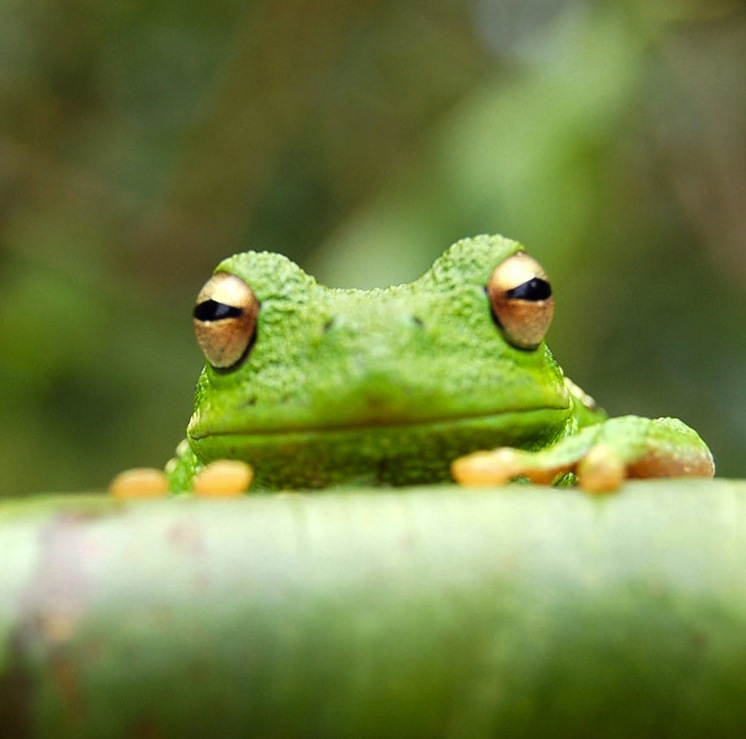
\includegraphics[width=0.5\textwidth]{frog.jpg}
% % \caption{\label{fig:frog}This is a figure caption.}
% % \end{figure}

% % \begin{table}
% % \centering
% % \begin{tabular}{l|r}
% % Item & Quantity \\\hline
% % Widgets & 42 \\
% % Gadgets & 13
% % \end{tabular}
% % \caption{\label{tab:widgets}An example table.}
% % \end{table}

% \subsection{Mathematics}

% \LaTeX{} is great at typesetting mathematics. Let $X_1, X_2, \ldots, X_n$ be a sequence of independent and identically distributed random variables with $\text{E}[X_i] = \mu$ and $\text{Var}[X_i] = \sigma^2 < \infty$, and let
% $$S_n = \frac{X_1 + X_2 + \cdots + X_n}{n}
%       = \frac{1}{n}\sum_{i}^{n} X_i$$
% denote their mean. Then as $n$ approaches infinity, the random variables $\sqrt{n}(S_n - \mu)$ converge in distribution to a normal $\mathcal{N}(0, \sigma^2)$.

% \subsection{Lists}

% You can make lists with automatic numbering \dots

% \begin{enumerate}
% \item Like this,
% \item and like this.
% \end{enumerate}
% \dots or bullet points \dots
% \begin{itemize}
% \item Like this,
% \item and like this.
% \end{itemize}

% We hope you find write\LaTeX\ useful, and please let us know if you have any feedback using the help menu above.

\end{document} to your LaTeX file where you want your
% title page.
%t
%%%%%%%%%%%%%%%%%%%%%%%%%%%%%%%%%%%%%%%%%
\title{Chatbot hỗ trợ thương mại điện tử}
%----------------------------------------------------------------------------------------
%	PACKAGES AND OTHER DOCUMENT CONFIGURATIONS
%----------------------------------------------------------------------------------------

\documentclass[12pt]{article}
\usepackage[T5]{fontenc}
\usepackage[utf8]{inputenc}
%\usepackage[utf8]{vietnam}
\usepackage{indentfirst} % thục dòng cái dòng đầu tiên 
\usepackage[vietnamese,english]{babel}
\usepackage{amsmath}
\usepackage{graphicx}
\usepackage[colorinlistoftodos]{todonotes}
\usepackage{listings}
\usepackage{xcolor}
\lstset{basicstyle=\ttfamily,
  showstringspaces=false,
%   commentstyle=\color{red},
%   keywordstyle=\color{blue}
}
\usepackage{hyperref}
\hypersetup{
    colorlinks=true,
    linkcolor=blue,
    filecolor=magenta,      
    urlcolor=cyan,
}


\renewcommand{\lstlistingname}{Mã }% Listing -> Algorithm
\addto\captionsenglish{\renewcommand{\figurename}{Hình}}

\begin{document}

\begin{titlepage}

\newcommand{\HRule}{\rule{\linewidth}{0.5mm}} % Defines a new command for the horizontal lines, change thickness here

\center % Center everything on the page
 
%----------------------------------------------------------------------------------------
%	HEADING SECTIONS
%----------------------------------------------------------------------------------------

\textsc{\LARGE Đại học Khoa học tự nhiên}\\[1.5cm] % Name of your university/college
\textsc{\Large Ngành hệ thống thông tin}\\[0.5cm] % Major heading such as course name
\textsc{\large Môn học: HỆ CƠ SỞ DỮ LIỆU NÂNG CAO }\\[0.5cm] % Minor heading such as course title

%----------------------------------------------------------------------------------------
%	TITLE SECTION
%----------------------------------------------------------------------------------------

\HRule \\[0.4cm]
{ \huge \bfseries 
Chatbot hỗ trợ thương mại điện tử
}\\[0.4cm] % Title of your document
\HRule \\[1.5cm]
 
%----------------------------------------------------------------------------------------
%	AUTHOR SECTION
%----------------------------------------------------------------------------------------

\begin{minipage}{0.5 \textwidth}
\begin{flushleft} \large
\emph{Học viên:}\\
Thái Thiện 17C12031 \\ % Your name
Lê Võ Minh Thư 17C12033
\end{flushleft}
\end{minipage}
~
\begin{minipage}{0.45 \textwidth}
\begin{flushright} \large
\emph{Giảng viên:} \\
TS. Nguyễn Trần Minh Thư % Supervisor's Name
\end{flushright}
\end{minipage}\\[1cm]

% If you don't want a supervisor, uncomment the two lines below and remove the section above
%\Large \emph{Author:}\\
%John \textsc{Smith}\\[3cm] % Your name

%----------------------------------------------------------------------------------------
%	DATE SECTION
%----------------------------------------------------------------------------------------

% I don't want day because it is English
% {\large \today}\\[2cm] % Date, change the \today to a set date if you want to be precise

%----------------------------------------------------------------------------------------
%	LOGO SECTION
%----------------------------------------------------------------------------------------


\includegraphics{logo/rsz_3logo-khtn.png}\\[1cm] % Include a department/university logo - this will require the graphicx package
 
%----------------------------------------------------------------------------------------

\vfill % Fill the rest of the page with whitespace

\end{titlepage}

\tableofcontents
\newpage

\section{Bài toán đặt ra}

\subsection{Chatbot}
	Chatbot là một hệ thống tự động có thể giao tiếp với người dùng để thực hiện các thao tác được lập trình sẵn.  Trong thương mại điện tử, Chatbot được dùng thay nhân viên trực tổng đài để tiếp khách hàng và giúp đỡ khách hàng một số tác vụ đơn giản như tìm kiếm sản phẩm. Từ đó giúp tiết kiệm nhân công, kênh liên lạc luôn thông suốt.
	

\subsection{Thông tin ứng dụng}

Trong đồ án này, nhóm chúng tôi xây dựng một chatbot cho trang thương mại điện tử "Xưởng may Thiên Phúc\footnote{\url{http://xuongmaythienphuc.vn/}}". Chatbot sẽ có tính năng chính là tìm kiếm và hiển thị thông tin sản phẩm. Mỗi sản phẩm trả về sẽ kèm đường dẫn tới trang thương mại điện tử, giúp khách hàng dễ dàng đăt hàng.


%%%%%%%%%%%%%%%%%%%%%START EXAMPLE THING%%%%%%%%%%%%%%%
% % % Commands to include a figure:
% \begin{figure}[h]
% \centering
% 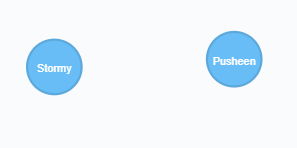
\includegraphics[width=0.5\textwidth]{image/node.PNG}
% \caption{\label{fig:node} Nút}
% \end{figure}


% % chuong 3
% \section{Chèn đoạn code}


% ví dụ code \ref{lst:vdcode} là code python 


% \begin{lstlisting}[caption={Đoạn code}, label={lst:vdcode}, language=python]
% s = "I am Pusheen the cat"
% print(s)
% \end{lstlisting}

% ví dụ trích dẫn \cite{robinson2013graph}
%%%%%%%%%%%%%% END EXAMPLE THING %%%%%%%%%%%%%%%%%%%%%%%%%

\section{Xây dựng ứng dụng}

\subsection{Mô hình hóa dữ liệu}

Dữ liệu nhập vào sẽ có dạng bảng có nhiều cột. Nhưng ta chỉ cần quan tâm 4 cột: Nhóm hàng, Mã hàng, Tên hàng, Giá bán. Dữ liệu cần nhập vào có bảng như dưới đây.

\begin{center}
 \begin{tabular}{||c c c c||} 
 \hline
 Nhóm hàng & Mã hàng & Tên hàng & Giá bán \\ [0.5ex] 
 \hline\hline
 Đồ Bộ Nữ & 1675NgoiXLSale & Set Bộ Dài Cam Ngói Phối Màu Sành Điệu & 120000 \\ 
 \hline
 Đầm dự tiệc & 1628DoXXLSale & Đầm đỏ body dự tiệc phối ren đuôi cá & 155000 \\
 \hline
  Đầm dự tiệc & 1573LSale & Đầm form chữ A tay ren cổ kết pha lê  & 120000 \\ [1ex] 
 \hline
\end{tabular}
\end{center}

Dữ liệu trong Neo4j sẽ có 4 thực thể: \pagebreak

\textbf{PRODUCT} : Sản phẩm 
\begin{itemize}
\item name (String) : Tên sản phẩm, lấy trực tiếp từ cột Tên Hàng trong bảng nguồn. 
\item normalized\_name (String) : Tên sản phẩm sau khi chuẩn hóa bằng cách bỏ dấu tiếng Việt và đổi sang viết thường. Chuẩn hóa giúp truy vấn tiếng Việt không dấu. 
\item url (String) : Đường dẫn tới sản phẩm trên trang "Xưởng may Thiên Phúc" 
\end{itemize}


\textbf{CATEGORY} : Nhóm hàng 
\begin{itemize}
\item name (String) : Tên nhóm hàng, lấy trực tiếp từ cột Nhóm hàng trong bảng nguồn
\item normalized\_name (String) : Tên nhóm hàng sau khi chuẩn hóa bằng cách bỏ dấu tiếng Việt và đổi sang viết thường. Chuẩn hóa giúp truy vấn tiếng Việt không dấu. 
\end{itemize}

\textbf{ITEM} : Mặt hàng. 
\begin{itemize}
\item code (String) : Mã hàng trong bảng nguồn. 
\item price (int) : giá tiền (đơn vị VND)  
\end{itemize}

Quan hệ giữa các thực thể 
\begin{itemize}
\item Một PRODUCT có từ 1 đến n quan hệ BELONG\_TO với CATEGORY
\item Một CATEGORY có từ 1 đến n quan hệ BELONG\_TO với PRODUCT
\item Một PRODUCT có từ 1 đến n quan hệ HAS với ITEM 
\item Một ITEM chỉ có 1 quan hệ HAS đến 1 PRODUCT 
\end{itemize}

Có thể diễn đạt bằng lời thế này: Mỗi sản phẩm thuộc nhiều nhóm hàng và có nhiều mặt hàng. Mội mặt hàng chỉ thuộc về một sản phẩm. 

Hình \ref{fig:datastructure} biểu diễn mối quan hệ giữa các thực thể. Hình \ref{fig:datastructureexample} biểu diễn trực quan hóa trên Neo4j gồm một CATEGORY (Nhóm hàng) với 2 PRODUCT (Sản phẩm) và các ITEM (mặt hàng) của mỗi sản phẩm.  

Chiều của quan hệ không ảnh hưởng đến quá trình nạp dữ liệu và truy vấn dữ liệu trong trường hợp sử dụng của đồ án này. 

% Commands to include a figure:
\begin{figure}[h]
\centering
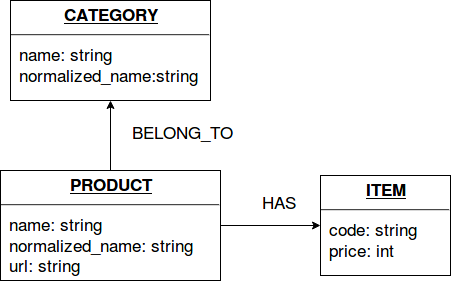
\includegraphics[width=0.5\textwidth]{image/neo4jdatastructure.png}
\caption{\label{fig:datastructure} Sơ đồ đồ quan hệ các thực thể}
\end{figure}


\begin{figure}[h]
\centering
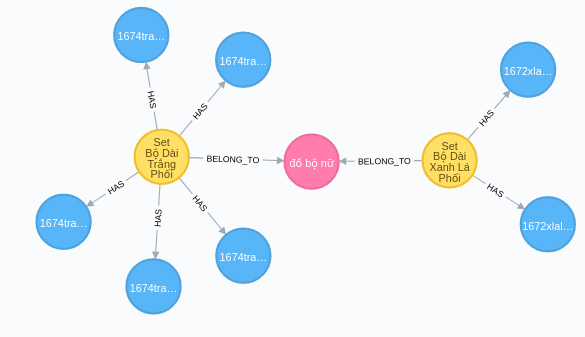
\includegraphics[width=0.5\textwidth]{imagev2/vddatamodel.png}
\caption{\label{fig:datastructureexample} Ví dụ đơn giản}
\end{figure}


\subsection{Chuyển đổi và nạp dữ liệu}
Chúng tôi chuyển đổi dữ liệu từ dạng bản sang các Neo4j Cypher, và dùng cypher đó để nạp vào cơ sở dữ liệu. Mã nguồn nằm trong thư mục csdlnc-util và hướng dẫn sử dụng được trình bày ở mục \ref{sec:csdlncutil}. Mỗi dòng trong bảng nguồn sẽ tạo ra 5 truy vấn. 

Các bước chuyển đổi: 
\begin{itemize}
\item Tạo CATEGORY 
\item Tạo PRODUCT 
\item Tạo ITEM
\item Tạo quan hệ BELONG\_TO giữa CATEGORY và PRODUCT 
\item Tạo quan hệ HAS giữa PRODUCT và ITEM
\end{itemize}

Ta lấy ví dụ, để nạp dòng đầu tiên vào Neo4j cần 5 truy vấn sau

\subsubsection{Tạo CATEGORY}\label{sec:mergecategory}
MERGE (category:CATEGORY{name: 'đồ bộ nữ', normalized\_name: 'do bo nu' })

Từ khóa MERGE sẽ tìm trong cơ sở dữ liệu thực thể CATEGORY như định nghĩa trong ngoặc tròn. Nếu không tìm được thực thể CATEGORY nào như định nghĩa, Neo4j sẽ tạo thực thể mới. Dùng MERGE thay CREATE sẽ giúp xử lý trường hợp trùng, lập nút. Ngoài ra, ở bước nạp dữ liệu, ta không cần xử lý query để xem Neo4j đã tồn tại thực thể đó chưa 

\subsubsection{Tạo PRODUCT}\label{sec:mergeproduct}

MERGE (product:PRODUCT{ name:'Set Bộ Dài Cam Ngói Phối Màu Sành Điệu', url: 'http://xuongmaythienphuc.vn/component/products/set-bo-dai-cam-ngoi-phoi-mau-sanh-dieu.html', normalized\_name: 'set bo dai cam ngoi phoi mau sanh dieu'})

\subsubsection{Tạo ITEM}\label{sec:mergeitem}

MERGE (item:ITEM{code:'1675ngoixlsale', price: 120000})

\subsubsection{Tạo mối quan hệ}\label{sec:mergerel}

\textit{Câu truy vấn tạo quan hệ BELONG\_TO:} 

\medskip

MATCH (category:CATEGORY), (product:PRODUCT) 

WHERE category.name = 'đồ bộ nữ' AND product.name = 'Set Bộ Dài Cam Ngói Phối Màu Sành Điệu'

MERGE (category)<-[:BELONG\_TO]-(product)

\bigskip

\textit{Câu truy vấn tạo quan hệ HAS:}

\medskip

MATCH (product:PRODUCT),(item:ITEM) 

WHERE  product.name = 'Set Bộ Dài Cam Ngói Phối Màu Sành Điệu' AND item.code = '1675ngoixlsale' 

MERGE (product)-[:HAS]->(item)

\bigskip

Một câu truy vấn có thể viết nhiều dòng. Nhưng mỗi dòng chỉ có thể chứa tối đa một câu truy vấn. Ta có thể nhập câu truy vấn nhiều dòng vào Neo4j Browser (Shift+Enter để xuống dòng, Ctrl + Enter để thực hiện truy vấn). Đối với các Neo4j driver, mỗi câu truy vấn là một chuỗi string có thể chứa dấu xuống hàng. Truy vấn nhiều hàng sau khi gộp lại một hàng có cùng ý nghĩa. 

\subsubsection{Gộp 5 câu truy vấn lại một câu truy vấn}
Có thể gộp cả 5 câu truy vấn trên thành 1 câu truy vấn duy nhất. Tuy nhiên, chúng tôi chưa áp dụng vào đồ án vì để giữ cho các câu truy vấn đơn giản, giúp dễ dàng gỡ lỗi khi cần thiết. Dưới đây là phương pháp gộp câu truy vấn. Phương pháp: 

\begin{itemize}
\item gộp 3 câu truy vấn MERGE tạo CATEGORY, PRODUCT, ITEM ở bước \ref{sec:mergecategory}, \ref{sec:mergeproduct}, \ref{sec:mergeitem}. 
\item bỏ vế MATCH và WHERE ở bước tạo quan hệ \ref{sec:mergerel}. 
\item gộp cả 5 MERGE lại (giữ nguyên thứ tự) thành câu truy vấn duy nhất 
\end{itemize} 

Ví dụ, trường hợp 5 câu truy vấn trên sẽ được gộp lại như sau

\medskip

MERGE (category:CATEGORY{name: 'đồ bộ nữ', normalized\_name: 'do bo nu' })

MERGE (product:PRODUCT{ name:'Set Bộ Dài Cam Ngói Phối Màu Sành Điệu', url: 'http://xuongmaythienphuc.vn/component/products/set-bo-dai-cam-ngoi-phoi-mau-sanh-dieu.html', normalized\_name: 'set bo dai cam ngoi phoi mau sanh dieu'})

MERGE (item:ITEM{code:'1675ngoixlsale', price: 120000})

MERGE (category)<-[:BELONG\_TO]-(product)

MERGE (product)-[:HAS]->(item)

\medskip

Giải thích: 3 vế MERGE đầu tiên không phụ thuộc vào định danh nào. Câu truy vấn tạo quan hệ phụ thuộc vào các định danh product, category, item. Khi đứng 1 mình, ta phải định nghĩa cho các định danh ấy bằng vế MATCH và WHERE. Tuy nhiên, khi gộp chung với các vế MERGE thì ta có thể tái sử dụng các định danh đã được định nghĩa ở các vế MERGE trên. Vì vậy, có thể bỏ các vế MATCH và WHERE. 

\bigskip

Sau khi chạy cả 5 truy vấn, hoặc một truy vấn gộp, ta đều được một đồ thị như hình \ref{fig:cypher} 

\begin{figure}[h]
\centering
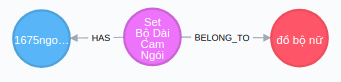
\includegraphics[width=0.5\textwidth]{imagev2/merge5cypher.png}
\caption{\label{fig:cypher} Đồ thị tạo ra từ dòng đầu tiên trong bảng nguồn}
\end{figure}

\subsection{Chatbot nền tảng Telegram}

Chatbot sẽ làm 2 việc sau: 

\begin{itemize}
\item Chuyển đổi đoạn chat của người dùng thành câu truy vấn 
\item Thực hiện truy vấn để lấy kết quả 
\item Xây dựng kết quả truy vấn thành câu trả lời cho người dùng 
\end{itemize}

Chatbot sẽ tiếp nhận yêu cầu của người dùng dưới dạng cú pháp bắt đầu bằng dấu gạch xiên "/". Khi đoạn chat không bắt đầu bằng dấu gạch xien "/" thì chatbot tự hiểu là tìm sản phẩm có tên là đoạn chat 

\subsubsection{/help} 
Hiển thị bản trợ giúp, bao gồm thông tin các câu lệnh

\subsubsection{/liet\_ke\_loai}
Liệt kê danh sách tất cả các nhóm hàng 

\subsubsection{/tim\_san\_pham <tên sản phẩm>}
Thực hiện tìm sản phẩm theo tên. Tên có thể viết có dấu hoặc không có dấu tiếng Việt. 
Câu truy vấn mẫu cho sản phẩm áo thun ("/tim\_san\_pham áo thun" hoặc "áo thun") như sau: 

\smallskip

MATCH (p:PRODUCT)-[:HAS]-(i:ITEM) 

WHERE p.name=~ '(?i).*áo thun.*' OR p.normalized\_name=~ '.*(?i)ao thun.*' 

RETURN p, i LIMIT 15

\smallskip

Ở về WHERE, dấu =~ sẽ kiểm tra các điều kiện thỏa Regular Expression (Regex) ghi trong dấu ngoặc kép. 
.*(?i)áo thun.* sẽ thỏa những câu có tồn tại từ "áo thun" (không phân biệt viết hoa, thường) trong cong. Vì vậy, vế WHERE này sẽ tìm những trường hợp mà nút PRODUCT có tên (hoặc tên không dấu) thỏa điều kiện của Regex  

Câu truy vấn trả về thông tin sản phẩm và mặt hàng 

\subsubsection{/tim\_loai <loại hoặc nhóm hàng> }

Tìm sản phẩm theo nhóm hàng.

Ví dụ: "/tim\_loai áo" sẽ tạo ra câu truy vấn sau
 
MATCH (c:CATEGORY)-[:BELONG\_TO]-(p:PRODUCT)

WHERE c.name=~'.*(?i)áo.*' OR c.normalized\_name=~'.*(?i)ao.*'  

return c, p

LIMIT 25

\smallskip

\subsubsection{/tim\_re\_hon <giá> và /tim\_mac\_hon <giá>}

Khi tìm sản phẩm theo giá, bot sẽ trả về sản phẩm gần với giá đó nhất, tùy theo người dùng muốn tìm rẻ hơn hay mắc hơn 

Ví dụ: truy vấn này tìm sản phẩm rẻ hơn 300 000 VND. Vế ORDER BY cùng từ khóa DESC sẽ xếp kết quả theo giá tiền từ cao đến thấp. Vì vậy, ta sẽ được sản phẩm gần với giá tiền ta tìm ở trên. 

MATCH (p:PRODUCT)-[:HAS]-(i:ITEM)

WHERE i.price <= 300000 

RETURN p, i 

ORDER BY i.price DESC 

LIMIT 15

\smallskip

Tương tự, bên dưới đây là ví dụ truy vấn của tìm sản phẩm mắc hơn 300000 VND. Trả về sẽ là các sản phẩm có mặt hàng có giá được xếp theo thứ tự từ 300 000 vnd trở lên. 

MATCH (p:PRODUCT)-[:HAS]-(i:ITEM)

WHERE i.price >= 300000 

RETURN p, i 

ORDER BY i.price  

LIMIT 15

\smallskip

\subsubsection{/re\_nhat và /mac\_nhat }

Trong 2 câu lệnh này, ta có thể thêm tên sản phẩm để lọc những sản phẩm có hoặc để trống tện sản phẩm để tìm với tất cả sản phẩm. 

"/re\_nhat" có câu truy vấn như sau: 

MATCH (p:PRODUCT)-[:HAS]-(i:ITEM)

return p, i 

ORDER BY i.price  

LIMIT 10

\smallskip

Dưới đây là truy vấn của "/mac\_nhat" 

MATCH (p:PRODUCT)-[:HAS]-(i:ITEM)

return p, i 

ORDER BY i.price DESC 

LIMIT 10

\smallskip

Nếu ta thêm vào tên sản phẩm, thì 2 truy vấn trên sẽ thêm vào vế WHERE để lọc kết quả theo tên sản phẩm. Dưới đây là ví dụ của truy vấn "/re\_nhat áo" 

MATCH (p:PRODUCT)-[:HAS]-(i:ITEM)

WHERE p.name=~ '.*(?i)áo.*' OR p.normalized\_name=~ '.*(?i)ao.*' 

RETURN p, i 

ORDER BY i.price  

LIMIT 10

\smallskip

Và "/mac\_nhat áo"

MATCH (p:PRODUCT)-[:HAS]-(i:ITEM)

WHERE p.name=~ '.*(?i)áo.*' OR p.normalized\_name=~ '.*(?i)ao.*' 

RETURN p, i 

ORDER BY i.price DESC 

LIMIT 10

\subsubsection{/tim\_khoang\_gia <chặn dưới> <chặn trên>}

Tìm khoảng giá sẽ trả về danh sách các sản phẩm có mặt hàng nằm trong khoảng giá đề ra. Ví dụ khi người dùng gửi tin nhắn "/tim\_khoang\_gia 200000 300000", bot sẽ tạo ra câu truy vấn sau 

MATCH (p:PRODUCT)-[:HAS]-(i:ITEM)  

WHERE i.price >= 200000 AND i.price <= 300000 

RETURN p, i 

ORDER BY i.price  

LIMIT 15

\subsubsection{/cung\_loai <mã sản phẩm>}

Chức năng này sẽ tìm sản phẩm cùng loại với sản phẩm mình đang quan tâm. Tin nhắn "/cung\_loai 816f" sẽ trả về các sản phẩm cùng loại với mặt hàng có mã 816f. Câu truy vấn được tạo ra như sau: 

MATCH (i:ITEM)-[:HAS]-(pp:PRODUCT)-[:BELONG\_TO]-(c:CATEGORY),

(c)-[:BELONG\_TO]-(p:PRODUCT)  

WHERE i.code = '816f'

RETURN p LIMIT 25



\subsubsection{Cách thức hiển thị kết quả từ câu truy vấn}

Truy vấn của câu lệnh /tim\_loai, /cung\_loai, sẽ trả chỉ trả về thông tin sản phẩm, Những truy vấn /tim\_san\_pham, /tim\_re\_hon, /tim\_mac\_hon, /tim\_re\_nhat, /tim\_mac\_nhat, /tim\_khoang\_gia sẽ trả về cả thông tin sản phẩm, mã mặt hàng và giá. 

Cụ thể như sau, với mỗi record của PRODUCT, bot sẽ hiển thị như sau: 

<Tên sản phẩm> <đường dẫn đến \url{http://xuongmaythienphuc.vn/}> 

\smallskip

Với mỗi record của ITEM, bot sẽ hiển thị 

<mã sản phẩm> <giá tiền> 

\smallskip 

Khi tồn tại cả PRODUCT và ITEM thì bot sẽ hiển thị tên sản phẩm, và các mã hàng - giá tiền thuộc sản phẩm đó, ví dụ như sau 

<Tên sản phẩm 1> <đường dẫn sp1> 
<mã sản phẩm 1.1> <giá tiền> 
<mã sản phẩm 1.2> <giá tiền> 
<Tên sản phẩm 2> <đường dẫn đến \url{http://xuongmaythienphuc.vn/}> 
<mã sản phẩm 2.1> <giá tiền> 
<mã sản phẩm 2.2> <giá tiền> 



\section{Triển khai ứng dụng}

\subsection{Cài đặt hệ thống}

Ứng dụng nên được triển khai trên hệ điều hành Ubuntu 18.04 LTS hoặc 16.04 LTS. Các yêu cầu: 

\begin{itemize}
\item Java (cài bằng sdkman \footnote{\url{https://sdkman.io/}})
\item gradle (cài bằng sdkman)
\item Python 3.6 (cài bằng Anaconda \footnote{\url{https://www.anaconda.com/download/}}hoặc Miniconda \footnote{\url{https://conda.io/miniconda.html}})
\end{itemize}

\subsection{Cài đặt và nạp dữ liệu vào Neo4j}
\subsubsection{Cài đặt Neo4j} \label{sec:installneo4jinstance}

Có 2 cách để cài đặt Neo4j: cài thông qua Neo4j Desktop hoặc cài trực tiếp Neo4j Community Edition

Tải bản Neo4j Desktop tại trang chủ \footnote{Tải về Neo4j Desktop https://neo4j.com/developer/guide-neo4j-desktop/} và cài đặt. Neo4j Desktop hỗ trợ những công cụ cần thiết để dựng một cơ sở dữ liệu trên máy cá nhân. Chạy Neo4j Desktop để tạo một graph database ở localhost (trên máy cá nhân). Phương pháp này chỉ nên dùng để thử nghiệm và sử dụng trong quá trình phát triển phần mềm, không nên dùng khi triển khai (Chạy thực tế)

Để cài đặt Neo4j Community Edition, làm theo hướng dẫn \footnote{https://neo4j.com/docs/operations-manual/current/installation/linux/debian/}. Cụ thể, chỉ cần chạy các câu lệnh sau (Mã \ref{lst:neo4jinstall})

\begin{lstlisting}[basicstyle=\tiny,language=bash,caption={Cài Neo4j},label={lst:neo4jinstall}]
wget -O - https://debian.neo4j.org/neotechnology.gpg.key | sudo apt-key add -
echo 'deb https://debian.neo4j.org/repo stable/' | sudo tee -a /etc/apt/sources.list.d/neo4j.list
sudo apt-get update
sudo apt-get install neo4j=1:3.4.5
\end{lstlisting}

\subsection{Nạp dữ liệu vào Neo4j}\label{sec:csdlncutil}

Dữ liệu thô từ trang thương mại điện tử có dạng Excel như sau: 

% TODO: gắn hình vào

Tập tin dữ liệu Excel nằm ở đường dẫn \url{csdlnc_util\\data\\DanhSachSanPham.xlsx}. Ta sẽ dùng các đoạn mã Python (thư mục csdlnc-util) để chuyển Excel thành Neo4j Cypher rồi chạy các cypher để nạp vào cơ sở dữ liệu. 

Yêu cầu các gói Python sau (có thể dùng câu lệnh pip install tên\_gói để cài đặt): 

\begin{itemize}
\item neo4j-driver
\item Unidecode 
\item openpyxl
\end{itemize}

Trước tiên, cần mỡ ex\_cypher\_file.py để thay đổi thông tin cơ sở dữ liệu. Tìm đoạn mã nguồn như Mã \ref{list:neo4jauth} và thay vào thông tin của Neo4j đã cài ở mục \ref{sec:installneo4jinstance}.

\begin{lstlisting}[language=python,caption={Thông tin Neo4j},label={list:neo4jauth}]
    uri = "bolt://188.166.233.199:7687"
    auth = ("tthien", "neo4jmeow")
\end{lstlisting}

Sau đó, chạy các dòng lệnh sau (Mã \ref{list:loadneo4jdata}) để nạp dữ liệu vào Neo4j.

\begin{lstlisting}[language=bash,caption={Cài Neo4j},label={list:loadneo4jdata}]
python import_product.py # chuyen Excel qua Cypher
python ex_cypher_file.py outcypher.txt # nap vao neo4j 
\end{lstlisting}

\subsection{Chatbot}
\subsubsection{Cài đặt tài khoản Bot trên Telegram}
Thực hiện các bước sau
\begin{itemize}
\item Tải ứng dụng Telegram vào điện thoại hoặc dùng bảng web \footnote{\url{https://web.telegram.org/}}
\item Tạo tài khoảng 
\item Liên hệ @BotFather \footnote{\url{https://t.me/botfather}} để tạo Bot và lấy API Token \footnote{API Token giống thế này: 681953844:AAF67DFPwTGuzHtPwZvGs1mjmLZ85IHTNmk}. 
\item Ghi lại tên bot và API Token 
\end{itemize}

\subsubsection{Chạy ứng dụng Chatbot}

Lần lượt chạy các đoạn Mã \ref{list:compiletelegrambot}, \ref{list:envtelegrambot}, \ref{list:runtelegrambot} để chạy bot. 

\begin{lstlisting}[language=bash,caption={Biên dịch mã nguồn},label={list:compiletelegrambot}]
gradle stage 
\end{lstlisting}

\begin{lstlisting}[language=bash,caption={Tạo các biến môi trường},label={list:envtelegrambot}]
export DEV_BOT_TOKEN=api_token
export DEV_BOT_NAME=ten_bot
export NEO4J_IP="localhost" 
export NEO4J_BOLT_PORT="7687"
export NEO4J_USERNAME="neo4j"
export NEO4J_PASSWORD=mat_khau_neo4j
\end{lstlisting}

\begin{lstlisting}[language=bash,caption={Chạy bot},label={list:runtelegrambot}]
java -jar build/libs/telegrambot-3.0-all.jar
\end{lstlisting}

\bibliographystyle{IEEEtran}
\bibliography{bib}

%%%%%%%%%%%%%%%%%%%%%%%%%%%%%%%%%%%%%%%%%%%%%%%%%%%%
% Comments can be added to the margins of the document using the \todo{Here's a comment in the margin!} todo command, as shown in the example on the right. You can also add inline comments too:

% \todo[inline, color=green!40]{This is an inline comment.}



% \subsection{Tables and Figures}

% Use the table and tabular commands for basic tables --- see Table~\ref{tab:widgets}, for example. You can upload a figure (JPEG, PNG or PDF) using the files menu. To include it in your document, use the includegraphics command as in the code for Figure~\ref{fig:frog} below.

% % % Commands to include a figure:
% % \begin{figure}
% % \centering
% % 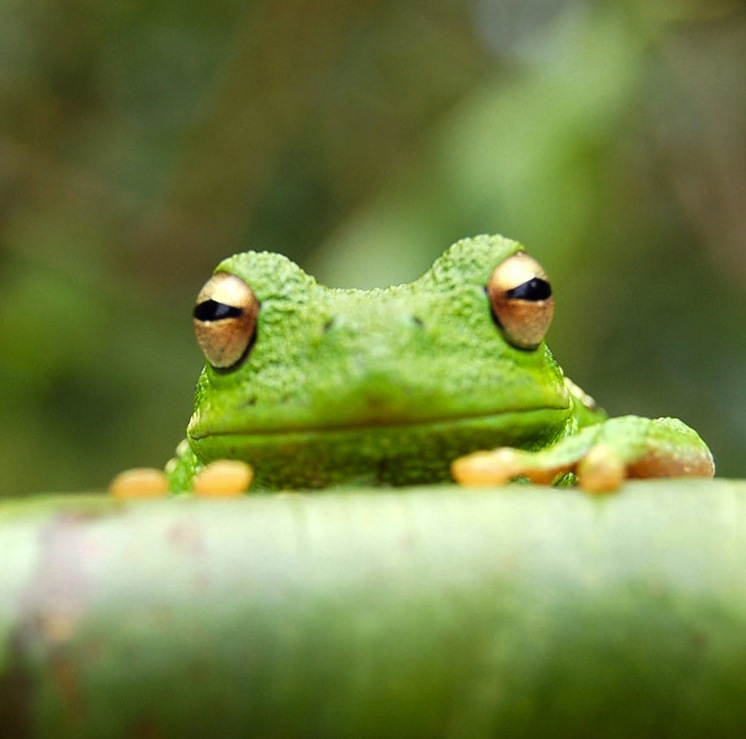
\includegraphics[width=0.5\textwidth]{frog.jpg}
% % \caption{\label{fig:frog}This is a figure caption.}
% % \end{figure}

% % \begin{table}
% % \centering
% % \begin{tabular}{l|r}
% % Item & Quantity \\\hline
% % Widgets & 42 \\
% % Gadgets & 13
% % \end{tabular}
% % \caption{\label{tab:widgets}An example table.}
% % \end{table}

% \subsection{Mathematics}

% \LaTeX{} is great at typesetting mathematics. Let $X_1, X_2, \ldots, X_n$ be a sequence of independent and identically distributed random variables with $\text{E}[X_i] = \mu$ and $\text{Var}[X_i] = \sigma^2 < \infty$, and let
% $$S_n = \frac{X_1 + X_2 + \cdots + X_n}{n}
%       = \frac{1}{n}\sum_{i}^{n} X_i$$
% denote their mean. Then as $n$ approaches infinity, the random variables $\sqrt{n}(S_n - \mu)$ converge in distribution to a normal $\mathcal{N}(0, \sigma^2)$.

% \subsection{Lists}

% You can make lists with automatic numbering \dots

% \begin{enumerate}
% \item Like this,
% \item and like this.
% \end{enumerate}
% \dots or bullet points \dots
% \begin{itemize}
% \item Like this,
% \item and like this.
% \end{itemize}

% We hope you find write\LaTeX\ useful, and please let us know if you have any feedback using the help menu above.

\end{document} to your LaTeX file where you want your
% title page.
%t
%%%%%%%%%%%%%%%%%%%%%%%%%%%%%%%%%%%%%%%%%
\title{Chatbot hỗ trợ thương mại điện tử}
%----------------------------------------------------------------------------------------
%	PACKAGES AND OTHER DOCUMENT CONFIGURATIONS
%----------------------------------------------------------------------------------------

\documentclass[12pt]{article}
\usepackage[T5]{fontenc}
\usepackage[utf8]{inputenc}
%\usepackage[utf8]{vietnam}
\usepackage{indentfirst} % thục dòng cái dòng đầu tiên 
\usepackage[vietnamese,english]{babel}
\usepackage{amsmath}
\usepackage{graphicx}
\usepackage[colorinlistoftodos]{todonotes}
\usepackage{listings}
\usepackage{xcolor}
\lstset{basicstyle=\ttfamily,
  showstringspaces=false,
%   commentstyle=\color{red},
%   keywordstyle=\color{blue}
}
\usepackage{hyperref}
\hypersetup{
    colorlinks=true,
    linkcolor=blue,
    filecolor=magenta,      
    urlcolor=cyan,
}


\renewcommand{\lstlistingname}{Mã }% Listing -> Algorithm
\addto\captionsenglish{\renewcommand{\figurename}{Hình}}

\begin{document}

\begin{titlepage}

\newcommand{\HRule}{\rule{\linewidth}{0.5mm}} % Defines a new command for the horizontal lines, change thickness here

\center % Center everything on the page
 
%----------------------------------------------------------------------------------------
%	HEADING SECTIONS
%----------------------------------------------------------------------------------------

\textsc{\LARGE Đại học Khoa học tự nhiên}\\[1.5cm] % Name of your university/college
\textsc{\Large Ngành hệ thống thông tin}\\[0.5cm] % Major heading such as course name
\textsc{\large Môn học: HỆ CƠ SỞ DỮ LIỆU NÂNG CAO }\\[0.5cm] % Minor heading such as course title

%----------------------------------------------------------------------------------------
%	TITLE SECTION
%----------------------------------------------------------------------------------------

\HRule \\[0.4cm]
{ \huge \bfseries 
Chatbot hỗ trợ thương mại điện tử
}\\[0.4cm] % Title of your document
\HRule \\[1.5cm]
 
%----------------------------------------------------------------------------------------
%	AUTHOR SECTION
%----------------------------------------------------------------------------------------

\begin{minipage}{0.5 \textwidth}
\begin{flushleft} \large
\emph{Học viên:}\\
Thái Thiện 17C12031 \\ % Your name
Lê Võ Minh Thư 17C12033
\end{flushleft}
\end{minipage}
~
\begin{minipage}{0.45 \textwidth}
\begin{flushright} \large
\emph{Giảng viên:} \\
TS. Nguyễn Trần Minh Thư % Supervisor's Name
\end{flushright}
\end{minipage}\\[1cm]

% If you don't want a supervisor, uncomment the two lines below and remove the section above
%\Large \emph{Author:}\\
%John \textsc{Smith}\\[3cm] % Your name

%----------------------------------------------------------------------------------------
%	DATE SECTION
%----------------------------------------------------------------------------------------

% I don't want day because it is English
% {\large \today}\\[2cm] % Date, change the \today to a set date if you want to be precise

%----------------------------------------------------------------------------------------
%	LOGO SECTION
%----------------------------------------------------------------------------------------


\includegraphics{logo/rsz_3logo-khtn.png}\\[1cm] % Include a department/university logo - this will require the graphicx package
 
%----------------------------------------------------------------------------------------

\vfill % Fill the rest of the page with whitespace

\end{titlepage}

\tableofcontents
\newpage

\section{Bài toán đặt ra}

\subsection{Chatbot}
	Chatbot là một hệ thống tự động có thể giao tiếp với người dùng để thực hiện các thao tác được lập trình sẵn.  Trong thương mại điện tử, Chatbot được dùng thay nhân viên trực tổng đài để tiếp khách hàng và giúp đỡ khách hàng một số tác vụ đơn giản như tìm kiếm sản phẩm. Từ đó giúp tiết kiệm nhân công, kênh liên lạc luôn thông suốt.
	

\subsection{Thông tin ứng dụng}

Trong đồ án này, nhóm chúng tôi xây dựng một chatbot cho trang thương mại điện tử "Xưởng may Thiên Phúc\footnote{\url{http://xuongmaythienphuc.vn/}}". Chatbot sẽ có tính năng chính là tìm kiếm và hiển thị thông tin sản phẩm. Mỗi sản phẩm trả về sẽ kèm đường dẫn tới trang thương mại điện tử, giúp khách hàng dễ dàng đăt hàng.


%%%%%%%%%%%%%%%%%%%%%START EXAMPLE THING%%%%%%%%%%%%%%%
% % % Commands to include a figure:
% \begin{figure}[h]
% \centering
% 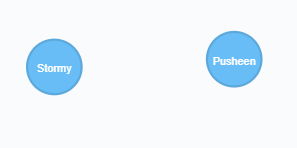
\includegraphics[width=0.5\textwidth]{image/node.PNG}
% \caption{\label{fig:node} Nút}
% \end{figure}


% % chuong 3
% \section{Chèn đoạn code}


% ví dụ code \ref{lst:vdcode} là code python 


% \begin{lstlisting}[caption={Đoạn code}, label={lst:vdcode}, language=python]
% s = "I am Pusheen the cat"
% print(s)
% \end{lstlisting}

% ví dụ trích dẫn \cite{robinson2013graph}
%%%%%%%%%%%%%% END EXAMPLE THING %%%%%%%%%%%%%%%%%%%%%%%%%

\section{Xây dựng ứng dụng}

\subsection{Mô hình hóa dữ liệu}

Dữ liệu nhập vào sẽ có dạng bảng có nhiều cột. Nhưng ta chỉ cần quan tâm 4 cột: Nhóm hàng, Mã hàng, Tên hàng, Giá bán. Dữ liệu cần nhập vào có bảng như dưới đây.

\begin{center}
 \begin{tabular}{||c c c c||} 
 \hline
 Nhóm hàng & Mã hàng & Tên hàng & Giá bán \\ [0.5ex] 
 \hline\hline
 Đồ Bộ Nữ & 1675NgoiXLSale & Set Bộ Dài Cam Ngói Phối Màu Sành Điệu & 120000 \\ 
 \hline
 Đầm dự tiệc & 1628DoXXLSale & Đầm đỏ body dự tiệc phối ren đuôi cá & 155000 \\
 \hline
  Đầm dự tiệc & 1573LSale & Đầm form chữ A tay ren cổ kết pha lê  & 120000 \\ [1ex] 
 \hline
\end{tabular}
\end{center}

Dữ liệu trong Neo4j sẽ có 4 thực thể: \pagebreak

\textbf{PRODUCT} : Sản phẩm 
\begin{itemize}
\item name (String) : Tên sản phẩm, lấy trực tiếp từ cột Tên Hàng trong bảng nguồn. 
\item normalized\_name (String) : Tên sản phẩm sau khi chuẩn hóa bằng cách bỏ dấu tiếng Việt và đổi sang viết thường. Chuẩn hóa giúp truy vấn tiếng Việt không dấu. 
\item url (String) : Đường dẫn tới sản phẩm trên trang "Xưởng may Thiên Phúc" 
\end{itemize}


\textbf{CATEGORY} : Nhóm hàng 
\begin{itemize}
\item name (String) : Tên nhóm hàng, lấy trực tiếp từ cột Nhóm hàng trong bảng nguồn
\item normalized\_name (String) : Tên nhóm hàng sau khi chuẩn hóa bằng cách bỏ dấu tiếng Việt và đổi sang viết thường. Chuẩn hóa giúp truy vấn tiếng Việt không dấu. 
\end{itemize}

\textbf{ITEM} : Mặt hàng. 
\begin{itemize}
\item code (String) : Mã hàng trong bảng nguồn. 
\item price (int) : giá tiền (đơn vị VND)  
\end{itemize}

Quan hệ giữa các thực thể 
\begin{itemize}
\item Một PRODUCT có từ 1 đến n quan hệ BELONG\_TO với CATEGORY
\item Một CATEGORY có từ 1 đến n quan hệ BELONG\_TO với PRODUCT
\item Một PRODUCT có từ 1 đến n quan hệ HAS với ITEM 
\item Một ITEM chỉ có 1 quan hệ HAS đến 1 PRODUCT 
\end{itemize}

Có thể diễn đạt bằng lời thế này: Mỗi sản phẩm thuộc nhiều nhóm hàng và có nhiều mặt hàng. Mội mặt hàng chỉ thuộc về một sản phẩm. 

Hình \ref{fig:datastructure} biểu diễn mối quan hệ giữa các thực thể. Hình \ref{fig:datastructureexample} biểu diễn trực quan hóa trên Neo4j gồm một CATEGORY (Nhóm hàng) với 2 PRODUCT (Sản phẩm) và các ITEM (mặt hàng) của mỗi sản phẩm.  

Chiều của quan hệ không ảnh hưởng đến quá trình nạp dữ liệu và truy vấn dữ liệu trong trường hợp sử dụng của đồ án này. 

% Commands to include a figure:
\begin{figure}[h]
\centering
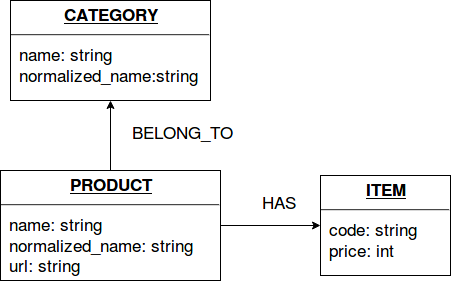
\includegraphics[width=0.5\textwidth]{image/neo4jdatastructure.png}
\caption{\label{fig:datastructure} Sơ đồ đồ quan hệ các thực thể}
\end{figure}


\begin{figure}[h]
\centering
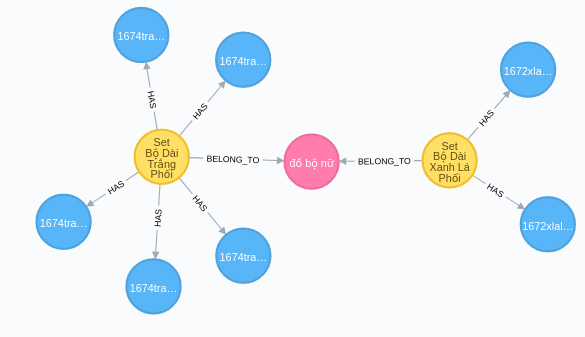
\includegraphics[width=0.5\textwidth]{imagev2/vddatamodel.png}
\caption{\label{fig:datastructureexample} Ví dụ đơn giản}
\end{figure}


\subsection{Chuyển đổi và nạp dữ liệu}
Chúng tôi chuyển đổi dữ liệu từ dạng bản sang các Neo4j Cypher, và dùng cypher đó để nạp vào cơ sở dữ liệu. Mã nguồn nằm trong thư mục csdlnc-util và hướng dẫn sử dụng được trình bày ở mục \ref{sec:csdlncutil}. Mỗi dòng trong bảng nguồn sẽ tạo ra 5 truy vấn. 

Các bước chuyển đổi: 
\begin{itemize}
\item Tạo CATEGORY 
\item Tạo PRODUCT 
\item Tạo ITEM
\item Tạo quan hệ BELONG\_TO giữa CATEGORY và PRODUCT 
\item Tạo quan hệ HAS giữa PRODUCT và ITEM
\end{itemize}

Ta lấy ví dụ, để nạp dòng đầu tiên vào Neo4j cần 5 truy vấn sau

\subsubsection{Tạo CATEGORY}\label{sec:mergecategory}
MERGE (category:CATEGORY{name: 'đồ bộ nữ', normalized\_name: 'do bo nu' })

Từ khóa MERGE sẽ tìm trong cơ sở dữ liệu thực thể CATEGORY như định nghĩa trong ngoặc tròn. Nếu không tìm được thực thể CATEGORY nào như định nghĩa, Neo4j sẽ tạo thực thể mới. Dùng MERGE thay CREATE sẽ giúp xử lý trường hợp trùng, lập nút. Ngoài ra, ở bước nạp dữ liệu, ta không cần xử lý query để xem Neo4j đã tồn tại thực thể đó chưa 

\subsubsection{Tạo PRODUCT}\label{sec:mergeproduct}

MERGE (product:PRODUCT{ name:'Set Bộ Dài Cam Ngói Phối Màu Sành Điệu', url: 'http://xuongmaythienphuc.vn/component/products/set-bo-dai-cam-ngoi-phoi-mau-sanh-dieu.html', normalized\_name: 'set bo dai cam ngoi phoi mau sanh dieu'})

\subsubsection{Tạo ITEM}\label{sec:mergeitem}

MERGE (item:ITEM{code:'1675ngoixlsale', price: 120000})

\subsubsection{Tạo mối quan hệ}\label{sec:mergerel}

\textit{Câu truy vấn tạo quan hệ BELONG\_TO:} 

\medskip

MATCH (category:CATEGORY), (product:PRODUCT) 

WHERE category.name = 'đồ bộ nữ' AND product.name = 'Set Bộ Dài Cam Ngói Phối Màu Sành Điệu'

MERGE (category)<-[:BELONG\_TO]-(product)

\bigskip

\textit{Câu truy vấn tạo quan hệ HAS:}

\medskip

MATCH (product:PRODUCT),(item:ITEM) 

WHERE  product.name = 'Set Bộ Dài Cam Ngói Phối Màu Sành Điệu' AND item.code = '1675ngoixlsale' 

MERGE (product)-[:HAS]->(item)

\bigskip

Một câu truy vấn có thể viết nhiều dòng. Nhưng mỗi dòng chỉ có thể chứa tối đa một câu truy vấn. Ta có thể nhập câu truy vấn nhiều dòng vào Neo4j Browser (Shift+Enter để xuống dòng, Ctrl + Enter để thực hiện truy vấn). Đối với các Neo4j driver, mỗi câu truy vấn là một chuỗi string có thể chứa dấu xuống hàng. Truy vấn nhiều hàng sau khi gộp lại một hàng có cùng ý nghĩa. 

\subsubsection{Gộp 5 câu truy vấn lại một câu truy vấn}
Có thể gộp cả 5 câu truy vấn trên thành 1 câu truy vấn duy nhất. Tuy nhiên, chúng tôi chưa áp dụng vào đồ án vì để giữ cho các câu truy vấn đơn giản, giúp dễ dàng gỡ lỗi khi cần thiết. Dưới đây là phương pháp gộp câu truy vấn. Phương pháp: 

\begin{itemize}
\item gộp 3 câu truy vấn MERGE tạo CATEGORY, PRODUCT, ITEM ở bước \ref{sec:mergecategory}, \ref{sec:mergeproduct}, \ref{sec:mergeitem}. 
\item bỏ vế MATCH và WHERE ở bước tạo quan hệ \ref{sec:mergerel}. 
\item gộp cả 5 MERGE lại (giữ nguyên thứ tự) thành câu truy vấn duy nhất 
\end{itemize} 

Ví dụ, trường hợp 5 câu truy vấn trên sẽ được gộp lại như sau

\medskip

MERGE (category:CATEGORY{name: 'đồ bộ nữ', normalized\_name: 'do bo nu' })

MERGE (product:PRODUCT{ name:'Set Bộ Dài Cam Ngói Phối Màu Sành Điệu', url: 'http://xuongmaythienphuc.vn/component/products/set-bo-dai-cam-ngoi-phoi-mau-sanh-dieu.html', normalized\_name: 'set bo dai cam ngoi phoi mau sanh dieu'})

MERGE (item:ITEM{code:'1675ngoixlsale', price: 120000})

MERGE (category)<-[:BELONG\_TO]-(product)

MERGE (product)-[:HAS]->(item)

\medskip

Giải thích: 3 vế MERGE đầu tiên không phụ thuộc vào định danh nào. Câu truy vấn tạo quan hệ phụ thuộc vào các định danh product, category, item. Khi đứng 1 mình, ta phải định nghĩa cho các định danh ấy bằng vế MATCH và WHERE. Tuy nhiên, khi gộp chung với các vế MERGE thì ta có thể tái sử dụng các định danh đã được định nghĩa ở các vế MERGE trên. Vì vậy, có thể bỏ các vế MATCH và WHERE. 

\bigskip

Sau khi chạy cả 5 truy vấn, hoặc một truy vấn gộp, ta đều được một đồ thị như hình \ref{fig:cypher} 

\begin{figure}[h]
\centering
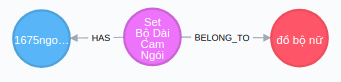
\includegraphics[width=0.5\textwidth]{imagev2/merge5cypher.png}
\caption{\label{fig:cypher} Đồ thị tạo ra từ dòng đầu tiên trong bảng nguồn}
\end{figure}

\subsection{Chatbot nền tảng Telegram}

Chatbot sẽ làm 2 việc sau: 

\begin{itemize}
\item Chuyển đổi đoạn chat của người dùng thành câu truy vấn 
\item Thực hiện truy vấn để lấy kết quả 
\item Xây dựng kết quả truy vấn thành câu trả lời cho người dùng 
\end{itemize}

Chatbot sẽ tiếp nhận yêu cầu của người dùng dưới dạng cú pháp bắt đầu bằng dấu gạch xiên "/". Khi đoạn chat không bắt đầu bằng dấu gạch xien "/" thì chatbot tự hiểu là tìm sản phẩm có tên là đoạn chat 

\subsubsection{/help} 
Hiển thị bản trợ giúp, bao gồm thông tin các câu lệnh

\subsubsection{/liet\_ke\_loai}
Liệt kê danh sách tất cả các nhóm hàng 

\subsubsection{/tim\_san\_pham <tên sản phẩm>}
Thực hiện tìm sản phẩm theo tên. Tên có thể viết có dấu hoặc không có dấu tiếng Việt. 
Câu truy vấn mẫu cho sản phẩm áo thun ("/tim\_san\_pham áo thun" hoặc "áo thun") như sau: 

\smallskip

MATCH (p:PRODUCT)-[:HAS]-(i:ITEM) 

WHERE p.name=~ '(?i).*áo thun.*' OR p.normalized\_name=~ '.*(?i)ao thun.*' 

RETURN p, i LIMIT 15

\smallskip

Ở về WHERE, dấu =~ sẽ kiểm tra các điều kiện thỏa Regular Expression (Regex) ghi trong dấu ngoặc kép. 
.*(?i)áo thun.* sẽ thỏa những câu có tồn tại từ "áo thun" (không phân biệt viết hoa, thường) trong cong. Vì vậy, vế WHERE này sẽ tìm những trường hợp mà nút PRODUCT có tên (hoặc tên không dấu) thỏa điều kiện của Regex  

Câu truy vấn trả về thông tin sản phẩm và mặt hàng 

\subsubsection{/tim\_loai <loại hoặc nhóm hàng> }

Tìm sản phẩm theo nhóm hàng.

Ví dụ: "/tim\_loai áo" sẽ tạo ra câu truy vấn sau
 
MATCH (c:CATEGORY)-[:BELONG\_TO]-(p:PRODUCT)

WHERE c.name=~'.*(?i)áo.*' OR c.normalized\_name=~'.*(?i)ao.*'  

return c, p

LIMIT 25

\smallskip

\subsubsection{/tim\_re\_hon <giá> và /tim\_mac\_hon <giá>}

Khi tìm sản phẩm theo giá, bot sẽ trả về sản phẩm gần với giá đó nhất, tùy theo người dùng muốn tìm rẻ hơn hay mắc hơn 

Ví dụ: truy vấn này tìm sản phẩm rẻ hơn 300 000 VND. Vế ORDER BY cùng từ khóa DESC sẽ xếp kết quả theo giá tiền từ cao đến thấp. Vì vậy, ta sẽ được sản phẩm gần với giá tiền ta tìm ở trên. 

MATCH (p:PRODUCT)-[:HAS]-(i:ITEM)

WHERE i.price <= 300000 

RETURN p, i 

ORDER BY i.price DESC 

LIMIT 15

\smallskip

Tương tự, bên dưới đây là ví dụ truy vấn của tìm sản phẩm mắc hơn 300000 VND. Trả về sẽ là các sản phẩm có mặt hàng có giá được xếp theo thứ tự từ 300 000 vnd trở lên. 

MATCH (p:PRODUCT)-[:HAS]-(i:ITEM)

WHERE i.price >= 300000 

RETURN p, i 

ORDER BY i.price  

LIMIT 15

\smallskip

\subsubsection{/re\_nhat và /mac\_nhat }

Trong 2 câu lệnh này, ta có thể thêm tên sản phẩm để lọc những sản phẩm có hoặc để trống tện sản phẩm để tìm với tất cả sản phẩm. 

"/re\_nhat" có câu truy vấn như sau: 

MATCH (p:PRODUCT)-[:HAS]-(i:ITEM)

return p, i 

ORDER BY i.price  

LIMIT 10

\smallskip

Dưới đây là truy vấn của "/mac\_nhat" 

MATCH (p:PRODUCT)-[:HAS]-(i:ITEM)

return p, i 

ORDER BY i.price DESC 

LIMIT 10

\smallskip

Nếu ta thêm vào tên sản phẩm, thì 2 truy vấn trên sẽ thêm vào vế WHERE để lọc kết quả theo tên sản phẩm. Dưới đây là ví dụ của truy vấn "/re\_nhat áo" 

MATCH (p:PRODUCT)-[:HAS]-(i:ITEM)

WHERE p.name=~ '.*(?i)áo.*' OR p.normalized\_name=~ '.*(?i)ao.*' 

RETURN p, i 

ORDER BY i.price  

LIMIT 10

\smallskip

Và "/mac\_nhat áo"

MATCH (p:PRODUCT)-[:HAS]-(i:ITEM)

WHERE p.name=~ '.*(?i)áo.*' OR p.normalized\_name=~ '.*(?i)ao.*' 

RETURN p, i 

ORDER BY i.price DESC 

LIMIT 10

\subsubsection{/tim\_khoang\_gia <chặn dưới> <chặn trên>}

Tìm khoảng giá sẽ trả về danh sách các sản phẩm có mặt hàng nằm trong khoảng giá đề ra. Ví dụ khi người dùng gửi tin nhắn "/tim\_khoang\_gia 200000 300000", bot sẽ tạo ra câu truy vấn sau 

MATCH (p:PRODUCT)-[:HAS]-(i:ITEM)  

WHERE i.price >= 200000 AND i.price <= 300000 

RETURN p, i 

ORDER BY i.price  

LIMIT 15

\subsubsection{/cung\_loai <mã sản phẩm>}

Chức năng này sẽ tìm sản phẩm cùng loại với sản phẩm mình đang quan tâm. Tin nhắn "/cung\_loai 816f" sẽ trả về các sản phẩm cùng loại với mặt hàng có mã 816f. Câu truy vấn được tạo ra như sau: 

MATCH (i:ITEM)-[:HAS]-(pp:PRODUCT)-[:BELONG\_TO]-(c:CATEGORY),

(c)-[:BELONG\_TO]-(p:PRODUCT)  

WHERE i.code = '816f'

RETURN p LIMIT 25



\subsubsection{Cách thức hiển thị kết quả từ câu truy vấn}

Truy vấn của câu lệnh /tim\_loai, /cung\_loai, sẽ trả chỉ trả về thông tin sản phẩm, Những truy vấn /tim\_san\_pham, /tim\_re\_hon, /tim\_mac\_hon, /tim\_re\_nhat, /tim\_mac\_nhat, /tim\_khoang\_gia sẽ trả về cả thông tin sản phẩm, mã mặt hàng và giá. 

Cụ thể như sau, với mỗi record của PRODUCT, bot sẽ hiển thị như sau: 

<Tên sản phẩm> <đường dẫn đến \url{http://xuongmaythienphuc.vn/}> 

\smallskip

Với mỗi record của ITEM, bot sẽ hiển thị 

<mã sản phẩm> <giá tiền> 

\smallskip 

Khi tồn tại cả PRODUCT và ITEM thì bot sẽ hiển thị tên sản phẩm, và các mã hàng - giá tiền thuộc sản phẩm đó, ví dụ như sau 

<Tên sản phẩm 1> <đường dẫn sp1> 
<mã sản phẩm 1.1> <giá tiền> 
<mã sản phẩm 1.2> <giá tiền> 
<Tên sản phẩm 2> <đường dẫn đến \url{http://xuongmaythienphuc.vn/}> 
<mã sản phẩm 2.1> <giá tiền> 
<mã sản phẩm 2.2> <giá tiền> 



\section{Triển khai ứng dụng}

\subsection{Cài đặt hệ thống}

Ứng dụng nên được triển khai trên hệ điều hành Ubuntu 18.04 LTS hoặc 16.04 LTS. Các yêu cầu: 

\begin{itemize}
\item Java (cài bằng sdkman \footnote{\url{https://sdkman.io/}})
\item gradle (cài bằng sdkman)
\item Python 3.6 (cài bằng Anaconda \footnote{\url{https://www.anaconda.com/download/}}hoặc Miniconda \footnote{\url{https://conda.io/miniconda.html}})
\end{itemize}

\subsection{Cài đặt và nạp dữ liệu vào Neo4j}
\subsubsection{Cài đặt Neo4j} \label{sec:installneo4jinstance}

Có 2 cách để cài đặt Neo4j: cài thông qua Neo4j Desktop hoặc cài trực tiếp Neo4j Community Edition

Tải bản Neo4j Desktop tại trang chủ \footnote{Tải về Neo4j Desktop https://neo4j.com/developer/guide-neo4j-desktop/} và cài đặt. Neo4j Desktop hỗ trợ những công cụ cần thiết để dựng một cơ sở dữ liệu trên máy cá nhân. Chạy Neo4j Desktop để tạo một graph database ở localhost (trên máy cá nhân). Phương pháp này chỉ nên dùng để thử nghiệm và sử dụng trong quá trình phát triển phần mềm, không nên dùng khi triển khai (Chạy thực tế)

Để cài đặt Neo4j Community Edition, làm theo hướng dẫn \footnote{https://neo4j.com/docs/operations-manual/current/installation/linux/debian/}. Cụ thể, chỉ cần chạy các câu lệnh sau (Mã \ref{lst:neo4jinstall})

\begin{lstlisting}[basicstyle=\tiny,language=bash,caption={Cài Neo4j},label={lst:neo4jinstall}]
wget -O - https://debian.neo4j.org/neotechnology.gpg.key | sudo apt-key add -
echo 'deb https://debian.neo4j.org/repo stable/' | sudo tee -a /etc/apt/sources.list.d/neo4j.list
sudo apt-get update
sudo apt-get install neo4j=1:3.4.5
\end{lstlisting}

\subsection{Nạp dữ liệu vào Neo4j}\label{sec:csdlncutil}

Dữ liệu thô từ trang thương mại điện tử có dạng Excel như sau: 

% TODO: gắn hình vào

Tập tin dữ liệu Excel nằm ở đường dẫn \url{csdlnc_util\\data\\DanhSachSanPham.xlsx}. Ta sẽ dùng các đoạn mã Python (thư mục csdlnc-util) để chuyển Excel thành Neo4j Cypher rồi chạy các cypher để nạp vào cơ sở dữ liệu. 

Yêu cầu các gói Python sau (có thể dùng câu lệnh pip install tên\_gói để cài đặt): 

\begin{itemize}
\item neo4j-driver
\item Unidecode 
\item openpyxl
\end{itemize}

Trước tiên, cần mỡ ex\_cypher\_file.py để thay đổi thông tin cơ sở dữ liệu. Tìm đoạn mã nguồn như Mã \ref{list:neo4jauth} và thay vào thông tin của Neo4j đã cài ở mục \ref{sec:installneo4jinstance}.

\begin{lstlisting}[language=python,caption={Thông tin Neo4j},label={list:neo4jauth}]
    uri = "bolt://188.166.233.199:7687"
    auth = ("tthien", "neo4jmeow")
\end{lstlisting}

Sau đó, chạy các dòng lệnh sau (Mã \ref{list:loadneo4jdata}) để nạp dữ liệu vào Neo4j.

\begin{lstlisting}[language=bash,caption={Cài Neo4j},label={list:loadneo4jdata}]
python import_product.py # chuyen Excel qua Cypher
python ex_cypher_file.py outcypher.txt # nap vao neo4j 
\end{lstlisting}

\subsection{Chatbot}
\subsubsection{Cài đặt tài khoản Bot trên Telegram}
Thực hiện các bước sau
\begin{itemize}
\item Tải ứng dụng Telegram vào điện thoại hoặc dùng bảng web \footnote{\url{https://web.telegram.org/}}
\item Tạo tài khoảng 
\item Liên hệ @BotFather \footnote{\url{https://t.me/botfather}} để tạo Bot và lấy API Token \footnote{API Token giống thế này: 681953844:AAF67DFPwTGuzHtPwZvGs1mjmLZ85IHTNmk}. 
\item Ghi lại tên bot và API Token 
\end{itemize}

\subsubsection{Chạy ứng dụng Chatbot}

Lần lượt chạy các đoạn Mã \ref{list:compiletelegrambot}, \ref{list:envtelegrambot}, \ref{list:runtelegrambot} để chạy bot. 

\begin{lstlisting}[language=bash,caption={Biên dịch mã nguồn},label={list:compiletelegrambot}]
gradle stage 
\end{lstlisting}

\begin{lstlisting}[language=bash,caption={Tạo các biến môi trường},label={list:envtelegrambot}]
export DEV_BOT_TOKEN=api_token
export DEV_BOT_NAME=ten_bot
export NEO4J_IP="localhost" 
export NEO4J_BOLT_PORT="7687"
export NEO4J_USERNAME="neo4j"
export NEO4J_PASSWORD=mat_khau_neo4j
\end{lstlisting}

\begin{lstlisting}[language=bash,caption={Chạy bot},label={list:runtelegrambot}]
java -jar build/libs/telegrambot-3.0-all.jar
\end{lstlisting}

\bibliographystyle{IEEEtran}
\bibliography{bib}

%%%%%%%%%%%%%%%%%%%%%%%%%%%%%%%%%%%%%%%%%%%%%%%%%%%%
% Comments can be added to the margins of the document using the \todo{Here's a comment in the margin!} todo command, as shown in the example on the right. You can also add inline comments too:

% \todo[inline, color=green!40]{This is an inline comment.}



% \subsection{Tables and Figures}

% Use the table and tabular commands for basic tables --- see Table~\ref{tab:widgets}, for example. You can upload a figure (JPEG, PNG or PDF) using the files menu. To include it in your document, use the includegraphics command as in the code for Figure~\ref{fig:frog} below.

% % % Commands to include a figure:
% % \begin{figure}
% % \centering
% % 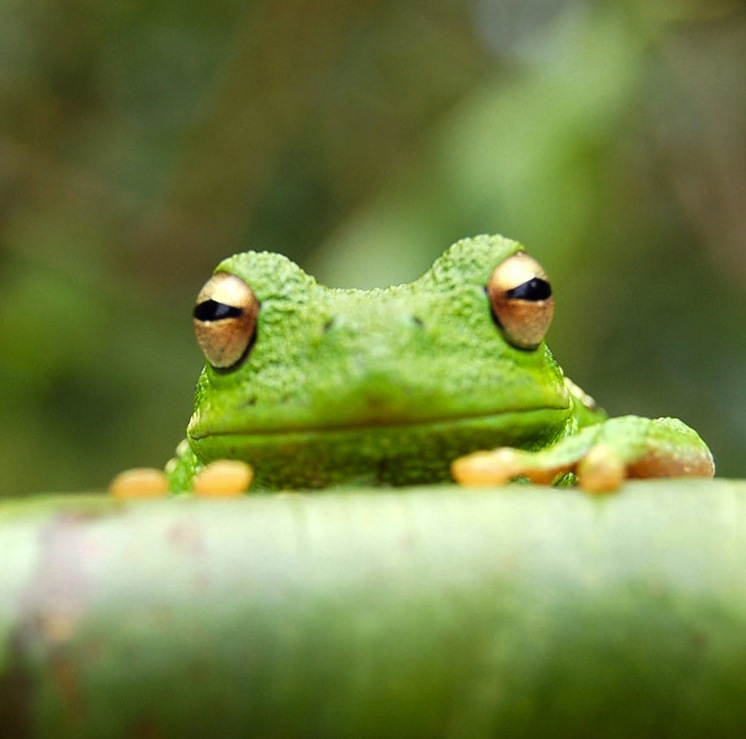
\includegraphics[width=0.5\textwidth]{frog.jpg}
% % \caption{\label{fig:frog}This is a figure caption.}
% % \end{figure}

% % \begin{table}
% % \centering
% % \begin{tabular}{l|r}
% % Item & Quantity \\\hline
% % Widgets & 42 \\
% % Gadgets & 13
% % \end{tabular}
% % \caption{\label{tab:widgets}An example table.}
% % \end{table}

% \subsection{Mathematics}

% \LaTeX{} is great at typesetting mathematics. Let $X_1, X_2, \ldots, X_n$ be a sequence of independent and identically distributed random variables with $\text{E}[X_i] = \mu$ and $\text{Var}[X_i] = \sigma^2 < \infty$, and let
% $$S_n = \frac{X_1 + X_2 + \cdots + X_n}{n}
%       = \frac{1}{n}\sum_{i}^{n} X_i$$
% denote their mean. Then as $n$ approaches infinity, the random variables $\sqrt{n}(S_n - \mu)$ converge in distribution to a normal $\mathcal{N}(0, \sigma^2)$.

% \subsection{Lists}

% You can make lists with automatic numbering \dots

% \begin{enumerate}
% \item Like this,
% \item and like this.
% \end{enumerate}
% \dots or bullet points \dots
% \begin{itemize}
% \item Like this,
% \item and like this.
% \end{itemize}

% We hope you find write\LaTeX\ useful, and please let us know if you have any feedback using the help menu above.

\end{document} to your LaTeX file where you want your
% title page.
%t
%%%%%%%%%%%%%%%%%%%%%%%%%%%%%%%%%%%%%%%%%
\title{Chatbot hỗ trợ thương mại điện tử}
%----------------------------------------------------------------------------------------
%	PACKAGES AND OTHER DOCUMENT CONFIGURATIONS
%----------------------------------------------------------------------------------------

\documentclass[12pt]{article}
\usepackage[T5]{fontenc}
\usepackage[utf8]{inputenc}
%\usepackage[utf8]{vietnam}
\usepackage{indentfirst} % thục dòng cái dòng đầu tiên 
\usepackage[vietnamese,english]{babel}
\usepackage{amsmath}
\usepackage{graphicx}
\usepackage[colorinlistoftodos]{todonotes}
\usepackage{listings}
\usepackage{float}  % force place image HERE with [H]
\usepackage{xcolor}
\lstset{basicstyle=\ttfamily,
  showstringspaces=false,
%   commentstyle=\color{red},
%   keywordstyle=\color{blue}
}
\usepackage{hyperref}
\hypersetup{
    colorlinks=true,
    linkcolor=blue,
    filecolor=magenta,      
    urlcolor=cyan,
}


\renewcommand{\lstlistingname}{Mã }% Listing -> Algorithm
\addto\captionsenglish{\renewcommand{\figurename}{Hình}}

\begin{document}

\begin{titlepage}

\newcommand{\HRule}{\rule{\linewidth}{0.5mm}} % Defines a new command for the horizontal lines, change thickness here

\center % Center everything on the page
 
%----------------------------------------------------------------------------------------
%	HEADING SECTIONS
%----------------------------------------------------------------------------------------

\textsc{\LARGE Đại học Khoa học tự nhiên}\\[1.5cm] % Name of your university/college
\textsc{\Large Ngành hệ thống thông tin}\\[0.5cm] % Major heading such as course name
\textsc{\large Môn học: HỆ CƠ SỞ DỮ LIỆU NÂNG CAO }\\[0.5cm] % Minor heading such as course title

%----------------------------------------------------------------------------------------
%	TITLE SECTION
%----------------------------------------------------------------------------------------

\HRule \\[0.4cm]
{ \huge \bfseries 
Chatbot hỗ trợ thương mại điện tử
}\\[0.4cm] % Title of your document
\HRule \\[1.5cm]
 
%----------------------------------------------------------------------------------------
%	AUTHOR SECTION
%----------------------------------------------------------------------------------------

\begin{minipage}{0.5 \textwidth}
\begin{flushleft} \large
\emph{Học viên:}\\
Thái Thiện 17C12031 \\ % Your name
Lê Võ Minh Thư 17C12033
\end{flushleft}
\end{minipage}
~
\begin{minipage}{0.45 \textwidth}
\begin{flushright} \large
\emph{Giảng viên:} \\
TS. Nguyễn Trần Minh Thư % Supervisor's Name
\end{flushright}
\end{minipage}\\[1cm]

% If you don't want a supervisor, uncomment the two lines below and remove the section above
%\Large \emph{Author:}\\
%John \textsc{Smith}\\[3cm] % Your name

%----------------------------------------------------------------------------------------
%	DATE SECTION
%----------------------------------------------------------------------------------------

% I don't want day because it is English
% {\large \today}\\[2cm] % Date, change the \today to a set date if you want to be precise

%----------------------------------------------------------------------------------------
%	LOGO SECTION
%----------------------------------------------------------------------------------------


\includegraphics{logo/rsz_3logo-khtn.png}\\[1cm] % Include a department/university logo - this will require the graphicx package
 
%----------------------------------------------------------------------------------------

\vfill % Fill the rest of the page with whitespace

\end{titlepage}

\tableofcontents
\newpage

\section{Bài toán đặt ra}

\subsection{Chatbot}
	Chatbot là một hệ thống tự động có thể giao tiếp với người dùng để thực hiện các thao tác được lập trình sẵn.  Trong thương mại điện tử, Chatbot được dùng thay nhân viên trực tổng đài để tiếp khách hàng và giúp đỡ khách hàng một số tác vụ đơn giản như tìm kiếm sản phẩm. Từ đó giúp tiết kiệm nhân công, kênh liên lạc luôn thông suốt \cite{lazarevich_2018}.
	

\subsection{Thông tin ứng dụng}

Trong đồ án này, nhóm chúng tôi xây dựng một chatbot cho trang thương mại điện tử "Xưởng may Thiên Phúc\footnote{\url{http://xuongmaythienphuc.vn/}}". Chatbot sẽ có tính năng chính là tìm kiếm và hiển thị thông tin sản phẩm. Mỗi sản phẩm trả về sẽ kèm đường dẫn tới trang thương mại điện tử, giúp khách hàng dễ dàng đăt hàng.

Cơ sở dữ liệu: Neo4j \cite{neo4j}

Nền tảng chat: Telegram \cite{telegrambot}

%%%%%%%%%%%%%%%%%%%%%START EXAMPLE THING%%%%%%%%%%%%%%%
% % % Commands to include a figure:
% \begin{figure}[h]
% \centering
% 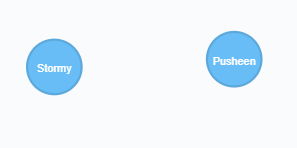
\includegraphics[width=0.5\textwidth]{image/node.PNG}
% \caption{\label{fig:node} Nút}
% \end{figure}


% % chuong 3
% \section{Chèn đoạn code}


% ví dụ code \ref{lst:vdcode} là code python 


% \begin{lstlisting}[caption={Đoạn code}, label={lst:vdcode}, language=python]
% s = "I am Pusheen the cat"
% print(s)
% \end{lstlisting}

% ví dụ trích dẫn \cite{robinson2013graph}
%%%%%%%%%%%%%% END EXAMPLE THING %%%%%%%%%%%%%%%%%%%%%%%%%

\section{Xây dựng ứng dụng}

\subsection{Mô hình hóa dữ liệu}

Dữ liệu nhập vào sẽ có dạng bảng có nhiều cột. Nhưng ta chỉ cần quan tâm 4 cột: Nhóm hàng, Mã hàng, Tên hàng, Giá bán. Dữ liệu cần nhập vào có bảng như dưới đây.

\begin{center}
 \begin{tabular}{||c c c c||} 
 \hline
 Nhóm hàng & Mã hàng & Tên hàng & Giá bán \\ [0.5ex] 
 \hline\hline
 Đồ Bộ Nữ & 1675NgoiXLSale & Set Bộ Dài Cam Ngói Phối Màu Sành Điệu & 120000 \\ 
 \hline
 Đầm dự tiệc & 1628DoXXLSale & Đầm đỏ body dự tiệc phối ren đuôi cá & 155000 \\
 \hline
  Đầm dự tiệc & 1573LSale & Đầm form chữ A tay ren cổ kết pha lê  & 120000 \\ [1ex] 
 \hline
\end{tabular}
\end{center}

Dữ liệu trong Neo4j sẽ có 4 thực thể: \pagebreak

\textbf{PRODUCT} : Sản phẩm 
\begin{itemize}
\item name (String) : Tên sản phẩm, lấy trực tiếp từ cột Tên Hàng trong bảng nguồn. 
\item normalized\_name (String) : Tên sản phẩm sau khi chuẩn hóa bằng cách bỏ dấu tiếng Việt và đổi sang viết thường. Chuẩn hóa giúp truy vấn tiếng Việt không dấu. 
\item url (String) : Đường dẫn tới sản phẩm trên trang "Xưởng may Thiên Phúc" 
\end{itemize}


\textbf{CATEGORY} : Nhóm hàng 
\begin{itemize}
\item name (String) : Tên nhóm hàng, lấy trực tiếp từ cột Nhóm hàng trong bảng nguồn
\item normalized\_name (String) : Tên nhóm hàng sau khi chuẩn hóa bằng cách bỏ dấu tiếng Việt và đổi sang viết thường. Chuẩn hóa giúp truy vấn tiếng Việt không dấu. 
\end{itemize}

\textbf{ITEM} : Mặt hàng. 
\begin{itemize}
\item code (String) : Mã hàng trong bảng nguồn. 
\item price (int) : giá tiền (đơn vị VND)  
\end{itemize}

Quan hệ giữa các thực thể 
\begin{itemize}
\item Một PRODUCT có từ 1 đến n quan hệ BELONG\_TO với CATEGORY
\item Một CATEGORY có từ 1 đến n quan hệ BELONG\_TO với PRODUCT
\item Một PRODUCT có từ 1 đến n quan hệ HAS với ITEM 
\item Một ITEM chỉ có 1 quan hệ HAS đến 1 PRODUCT 
\end{itemize}

Có thể diễn đạt bằng lời thế này: Mỗi sản phẩm thuộc nhiều nhóm hàng và có nhiều mặt hàng. Mội mặt hàng chỉ thuộc về một sản phẩm. 

Hình \ref{fig:datastructure} biểu diễn mối quan hệ giữa các thực thể. Hình \ref{fig:datastructureexample} biểu diễn trực quan hóa trên Neo4j gồm một CATEGORY (Nhóm hàng) với 2 PRODUCT (Sản phẩm) và các ITEM (mặt hàng) của mỗi sản phẩm.  

Chiều của quan hệ không ảnh hưởng đến quá trình nạp dữ liệu và truy vấn dữ liệu trong trường hợp sử dụng của đồ án này. 

% Commands to include a figure:
\begin{figure}[h]
\centering
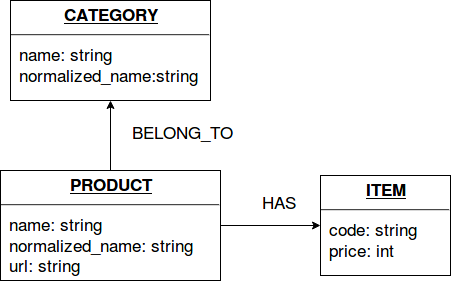
\includegraphics[width=0.5\textwidth]{image/neo4jdatastructure.png}
\caption{\label{fig:datastructure} Sơ đồ đồ quan hệ các thực thể}
\end{figure}


\begin{figure}[h]
\centering
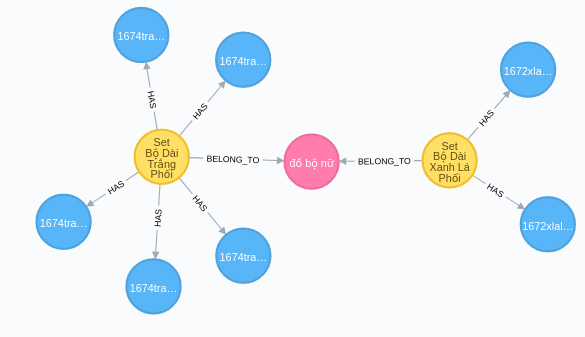
\includegraphics[width=0.5\textwidth]{imagev2/vddatamodel.png}
\caption{\label{fig:datastructureexample} Ví dụ đơn giản}
\end{figure}


\subsection{Chuyển đổi và nạp dữ liệu}
Chúng tôi chuyển đổi dữ liệu từ dạng bản sang các Neo4j Cypher, và dùng cypher đó để nạp vào cơ sở dữ liệu. Mã nguồn nằm trong thư mục csdlnc-util và hướng dẫn sử dụng được trình bày ở mục \ref{sec:csdlncutil}. Mỗi dòng trong bảng nguồn sẽ tạo ra 5 truy vấn. 

Các bước chuyển đổi: 
\begin{itemize}
\item Tạo CATEGORY 
\item Tạo PRODUCT 
\item Tạo ITEM
\item Tạo quan hệ BELONG\_TO giữa CATEGORY và PRODUCT 
\item Tạo quan hệ HAS giữa PRODUCT và ITEM
\end{itemize}

Ta lấy ví dụ, để nạp dòng đầu tiên vào Neo4j cần 5 truy vấn sau

\subsubsection{Tạo CATEGORY}\label{sec:mergecategory}
MERGE (category:CATEGORY{name: 'đồ bộ nữ', normalized\_name: 'do bo nu' })

Từ khóa MERGE sẽ tìm trong cơ sở dữ liệu thực thể CATEGORY như định nghĩa trong ngoặc tròn. Nếu không tìm được thực thể CATEGORY nào như định nghĩa, Neo4j sẽ tạo thực thể mới. Dùng MERGE thay CREATE sẽ giúp xử lý trường hợp trùng, lập nút. Ngoài ra, ở bước nạp dữ liệu, ta không cần xử lý query để xem Neo4j đã tồn tại thực thể đó chưa 

\subsubsection{Tạo PRODUCT}\label{sec:mergeproduct}

MERGE (product:PRODUCT{ name:'Set Bộ Dài Cam Ngói Phối Màu Sành Điệu', url: 'http://xuongmaythienphuc.vn/component/products/set-bo-dai-cam-ngoi-phoi-mau-sanh-dieu.html', normalized\_name: 'set bo dai cam ngoi phoi mau sanh dieu'})

\subsubsection{Tạo ITEM}\label{sec:mergeitem}

MERGE (item:ITEM{code:'1675ngoixlsale', price: 120000})

\subsubsection{Tạo mối quan hệ}\label{sec:mergerel}

\textit{Câu truy vấn tạo quan hệ BELONG\_TO:} 

\medskip

MATCH (category:CATEGORY), (product:PRODUCT) 

WHERE category.name = 'đồ bộ nữ' AND product.name = 'Set Bộ Dài Cam Ngói Phối Màu Sành Điệu'

MERGE (category)<-[:BELONG\_TO]-(product)

\bigskip

\textit{Câu truy vấn tạo quan hệ HAS:}

\medskip

MATCH (product:PRODUCT),(item:ITEM) 

WHERE  product.name = 'Set Bộ Dài Cam Ngói Phối Màu Sành Điệu' AND item.code = '1675ngoixlsale' 

MERGE (product)-[:HAS]->(item)

\bigskip

Một câu truy vấn có thể viết nhiều dòng. Nhưng mỗi dòng chỉ có thể chứa tối đa một câu truy vấn. Ta có thể nhập câu truy vấn nhiều dòng vào Neo4j Browser (Shift+Enter để xuống dòng, Ctrl + Enter để thực hiện truy vấn). Đối với các Neo4j driver, mỗi câu truy vấn là một chuỗi string có thể chứa dấu xuống hàng. Truy vấn nhiều hàng sau khi gộp lại một hàng có cùng ý nghĩa. 

\subsubsection{Gộp 5 câu truy vấn lại một câu truy vấn}
Có thể gộp cả 5 câu truy vấn trên thành 1 câu truy vấn duy nhất. Tuy nhiên, chúng tôi chưa áp dụng vào đồ án vì để giữ cho các câu truy vấn đơn giản, giúp dễ dàng gỡ lỗi khi cần thiết. Dưới đây là phương pháp gộp câu truy vấn. Phương pháp: 

\begin{itemize}
\item gộp 3 câu truy vấn MERGE tạo CATEGORY, PRODUCT, ITEM ở bước \ref{sec:mergecategory}, \ref{sec:mergeproduct}, \ref{sec:mergeitem}. 
\item bỏ vế MATCH và WHERE ở bước tạo quan hệ \ref{sec:mergerel}. 
\item gộp cả 5 MERGE lại (giữ nguyên thứ tự) thành câu truy vấn duy nhất 
\end{itemize} 

Ví dụ, trường hợp 5 câu truy vấn trên sẽ được gộp lại như sau

\medskip

MERGE (category:CATEGORY{name: 'đồ bộ nữ', normalized\_name: 'do bo nu' })

MERGE (product:PRODUCT{ name:'Set Bộ Dài Cam Ngói Phối Màu Sành Điệu', url: 'http://xuongmaythienphuc.vn/component/products/set-bo-dai-cam-ngoi-phoi-mau-sanh-dieu.html', normalized\_name: 'set bo dai cam ngoi phoi mau sanh dieu'})

MERGE (item:ITEM{code:'1675ngoixlsale', price: 120000})

MERGE (category)<-[:BELONG\_TO]-(product)

MERGE (product)-[:HAS]->(item)

\medskip

Giải thích: 3 vế MERGE đầu tiên không phụ thuộc vào định danh nào. Câu truy vấn tạo quan hệ phụ thuộc vào các định danh product, category, item. Khi đứng 1 mình, ta phải định nghĩa cho các định danh ấy bằng vế MATCH và WHERE. Tuy nhiên, khi gộp chung với các vế MERGE thì ta có thể tái sử dụng các định danh đã được định nghĩa ở các vế MERGE trên. Vì vậy, có thể bỏ các vế MATCH và WHERE. 

\bigskip

Sau khi chạy cả 5 truy vấn, hoặc một truy vấn gộp, ta đều được một đồ thị như hình \ref{fig:cypher} 

\begin{figure}[h]
\centering
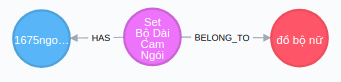
\includegraphics[width=0.5\textwidth]{imagev2/merge5cypher.png}
\caption{\label{fig:cypher} Đồ thị tạo ra từ dòng đầu tiên trong bảng nguồn}
\end{figure}

\subsubsection{Tạo URL và lọc dữ liệu}

Trước khi chuyển đổi thành các câu truy vấn, mỗi dòng, tên sản phẩm được dùng để tạo ra URL . Cách tạo như sau: 

\begin{itemize}
\item Từ tên sản phẩm, bỏ dấu tiếng Việt và chuyển sang viết thường 
\item Thay khoảng trắng " " bằng dấu gạch "-" 
\item Thêm tiền tố  \url{http://xuongmaythienphuc.vn/component/products/}.
\item Thêm hậu tố ".html"
\end{itemize}

Ví dụ: 

Tên sản phẩm "Áo Sơ Mi Trắng Thời Trang Hè 2018" chuyển thành "http://xuongmaythienphuc.vn/component/products/ao-so-mi-trang-thoi-trang-he-2018.html". Sau đó, url sẽ được truy cập để kiểm tra, nếu trả về với mã 200 , thì dòng đó trong excel mới được xử lý tiếp để tạo ra câu truy vấn. 

Dữ liệu Excel có 4725 dòng. Sau khi nạp vào Neo4j, tạo ra 

\begin{itemize}
\item 12 nút CATEGORY 
\item 477 nút PRODUCT 
\item 1195 nút ITEM 
\item 736 quan hệ BELONG\_TO 
\item 1195 quan hệ HAS 
\end{itemize}



\subsection{Chatbot nền tảng Telegram}

Chatbot sẽ làm 2 việc sau: 

\begin{itemize}
\item Chuyển đổi đoạn chat của người dùng thành câu truy vấn 
\item Thực hiện truy vấn để lấy kết quả 
\item Xây dựng kết quả truy vấn thành câu trả lời cho người dùng 
\end{itemize}

Chatbot sẽ tiếp nhận yêu cầu của người dùng dưới dạng cú pháp bắt đầu bằng dấu gạch xiên "/". Khi đoạn chat không bắt đầu bằng dấu gạch xien "/" thì chatbot tự hiểu là tìm sản phẩm có tên là đoạn chat.

Lúc đầu có 4275 dòng excel. Sau khi nạp vào Neo4j, tạo ra 

\subsubsection{/help} 
Hiển thị bản trợ giúp, bao gồm thông tin các câu lệnh

\subsubsection{/liet\_ke\_loai}
Liệt kê danh sách tất cả các nhóm hàng 

\subsubsection{/tim\_san\_pham <tên sản phẩm>}
Thực hiện tìm sản phẩm theo tên. Tên có thể viết có dấu hoặc không có dấu tiếng Việt. 
Câu truy vấn mẫu cho sản phẩm áo thun ("/tim\_san\_pham áo thun" hoặc "áo thun") như sau: 

\smallskip

MATCH (p:PRODUCT)-[:HAS]-(i:ITEM) 

WHERE p.name=~ '(?i).*áo thun.*' OR p.normalized\_name=~ '.*(?i)ao thun.*' 

RETURN p, i LIMIT 15

\smallskip

Ở về WHERE, dấu =~ sẽ kiểm tra các điều kiện thỏa Regular Expression (Regex) ghi trong dấu ngoặc kép. 
.*(?i)áo thun.* sẽ thỏa những câu có tồn tại từ "áo thun" (không phân biệt viết hoa, thường) trong cong. Vì vậy, vế WHERE này sẽ tìm những trường hợp mà nút PRODUCT có tên (hoặc tên không dấu) thỏa điều kiện của Regex  

Câu truy vấn trả về thông tin sản phẩm và mặt hàng 

\subsubsection{/tim\_loai <loại hoặc nhóm hàng> }

Tìm sản phẩm theo nhóm hàng.

Ví dụ: "/tim\_loai áo" sẽ tạo ra câu truy vấn sau
 
MATCH (c:CATEGORY)-[:BELONG\_TO]-(p:PRODUCT)

WHERE c.name=~'.*(?i)áo.*' OR c.normalized\_name=~'.*(?i)ao.*'  

return c, p

LIMIT 25

\smallskip

\subsubsection{/tim\_re\_hon <giá> và /tim\_mac\_hon <giá>}

Khi tìm sản phẩm theo giá, bot sẽ trả về sản phẩm gần với giá đó nhất, tùy theo người dùng muốn tìm rẻ hơn hay mắc hơn 

Ví dụ: truy vấn này tìm sản phẩm rẻ hơn 300 000 VND. Vế ORDER BY cùng từ khóa DESC sẽ xếp kết quả theo giá tiền từ cao đến thấp. Vì vậy, ta sẽ được sản phẩm gần với giá tiền ta tìm ở trên. 

MATCH (p:PRODUCT)-[:HAS]-(i:ITEM)

WHERE i.price <= 300000 

RETURN p, i 

ORDER BY i.price DESC 

LIMIT 15

\smallskip

Tương tự, bên dưới đây là ví dụ truy vấn của tìm sản phẩm mắc hơn 300000 VND. Trả về sẽ là các sản phẩm có mặt hàng có giá được xếp theo thứ tự từ 300 000 vnd trở lên. 

MATCH (p:PRODUCT)-[:HAS]-(i:ITEM)

WHERE i.price >= 300000 

RETURN p, i 

ORDER BY i.price  

LIMIT 15

\smallskip

\subsubsection{/re\_nhat và /mac\_nhat }

Trong 2 câu lệnh này, ta có thể thêm tên sản phẩm để lọc những sản phẩm có hoặc để trống tện sản phẩm để tìm với tất cả sản phẩm. 

"/re\_nhat" có câu truy vấn như sau: 

MATCH (p:PRODUCT)-[:HAS]-(i:ITEM)

return p, i 

ORDER BY i.price  

LIMIT 10

\smallskip

Dưới đây là truy vấn của "/mac\_nhat" 

MATCH (p:PRODUCT)-[:HAS]-(i:ITEM)

return p, i 

ORDER BY i.price DESC 

LIMIT 10

\smallskip

Nếu ta thêm vào tên sản phẩm, thì 2 truy vấn trên sẽ thêm vào vế WHERE để lọc kết quả theo tên sản phẩm. Dưới đây là ví dụ của truy vấn "/re\_nhat áo" 

MATCH (p:PRODUCT)-[:HAS]-(i:ITEM)

WHERE p.name=~ '.*(?i)áo.*' OR p.normalized\_name=~ '.*(?i)ao.*' 

RETURN p, i 

ORDER BY i.price  

LIMIT 10

\smallskip

Và "/mac\_nhat áo"

MATCH (p:PRODUCT)-[:HAS]-(i:ITEM)

WHERE p.name=~ '.*(?i)áo.*' OR p.normalized\_name=~ '.*(?i)ao.*' 

RETURN p, i 

ORDER BY i.price DESC 

LIMIT 10

\subsubsection{/tim\_khoang\_gia <chặn dưới> <chặn trên>}

Tìm khoảng giá sẽ trả về danh sách các sản phẩm có mặt hàng nằm trong khoảng giá đề ra. Ví dụ khi người dùng gửi tin nhắn "/tim\_khoang\_gia 200000 300000", bot sẽ tạo ra câu truy vấn sau 

MATCH (p:PRODUCT)-[:HAS]-(i:ITEM)  

WHERE i.price >= 200000 AND i.price <= 300000 

RETURN p, i 

ORDER BY i.price  

LIMIT 15

\subsubsection{/cung\_loai <mã sản phẩm>}

Chức năng này sẽ tìm sản phẩm cùng loại với sản phẩm mình đang quan tâm. Tin nhắn "/cung\_loai 816f" sẽ trả về các sản phẩm cùng loại với mặt hàng có mã 816f. Câu truy vấn được tạo ra như sau: 

MATCH (i:ITEM)-[:HAS]-(pp:PRODUCT)-[:BELONG\_TO]-(c:CATEGORY),

(c)-[:BELONG\_TO]-(p:PRODUCT)  

WHERE i.code = '816f'

RETURN p LIMIT 25



\subsubsection{Cách thức hiển thị kết quả từ câu truy vấn}

Truy vấn của câu lệnh /tim\_loai, /cung\_loai, sẽ trả chỉ trả về thông tin sản phẩm, Những truy vấn /tim\_san\_pham, /tim\_re\_hon, /tim\_mac\_hon, /tim\_re\_nhat, /tim\_mac\_nhat, /tim\_khoang\_gia sẽ trả về cả thông tin sản phẩm, mã mặt hàng và giá. 

Cụ thể như sau, với mỗi record của PRODUCT, bot sẽ hiển thị như sau: 

<Tên sản phẩm> <đường dẫn đến \url{http://xuongmaythienphuc.vn/}> 

\smallskip

Với mỗi record của ITEM, bot sẽ hiển thị 

<mã sản phẩm> <giá tiền> 

\smallskip 

Khi tồn tại cả PRODUCT và ITEM thì bot sẽ hiển thị tên sản phẩm, và các mã hàng - giá tiền thuộc sản phẩm đó, ví dụ như sau 

<Tên sản phẩm 1> <đường dẫn sp1> 

<mã sản phẩm 1.1> <giá tiền> 

<mã sản phẩm 1.2> <giá tiền> 

<Tên sản phẩm 2> <đường dẫn đến \url{http://xuongmaythienphuc.vn/}> 

<mã sản phẩm 2.1> <giá tiền> 

<mã sản phẩm 2.2> <giá tiền> 

Hình \ref{fig:displayproduct} và hình \ref{fig:displayproductitem} minh họa cách hiển thị thông tin của chatbot. 

\begin{figure}[H]
\centering
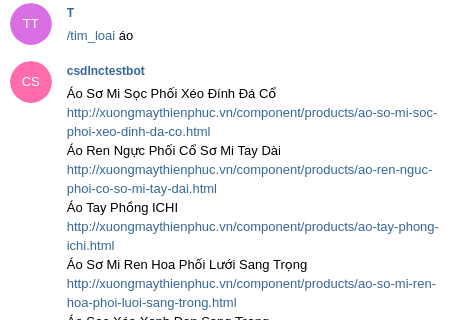
\includegraphics[width=0.9\textwidth]{imagev2/displayproduct.png}
\caption{\label{fig:displayproduct} Chỉ hiển thị sản phẩm}
\end{figure}

\begin{figure}[H]
\centering
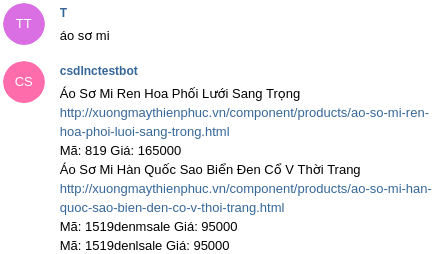
\includegraphics[width=0.8\textwidth]{imagev2/displayproductitem.png}
\caption{\label{fig:displayproductitem} hiển thị sản phẩm kèm giá }
\end{figure}

\section{Triển khai ứng dụng}

\subsection{Cài đặt hệ thống}

Ứng dụng nên được triển khai trên hệ điều hành Ubuntu 18.04 LTS hoặc 16.04 LTS. Các yêu cầu: 

\begin{itemize}
\item Java (cài bằng sdkman \footnote{\url{https://sdkman.io/}})
\item gradle (cài bằng sdkman)
\item Python 3.6 (cài bằng Anaconda \footnote{\url{https://www.anaconda.com/download/}}hoặc Miniconda \footnote{\url{https://conda.io/miniconda.html}})
\end{itemize}

\subsection{Cài đặt và nạp dữ liệu vào Neo4j}
\subsubsection{Cài đặt Neo4j} \label{sec:installneo4jinstance}

Có 2 cách để cài đặt Neo4j: cài thông qua Neo4j Desktop hoặc cài trực tiếp Neo4j Community Edition

Tải bản Neo4j Desktop tại trang chủ \footnote{Tải về Neo4j Desktop https://neo4j.com/developer/guide-neo4j-desktop/} và cài đặt. Neo4j Desktop hỗ trợ những công cụ cần thiết để dựng một cơ sở dữ liệu trên máy cá nhân. Chạy Neo4j Desktop để tạo một graph database ở localhost (trên máy cá nhân). Phương pháp này chỉ nên dùng để thử nghiệm và sử dụng trong quá trình phát triển phần mềm, không nên dùng khi triển khai (Chạy thực tế)

Để cài đặt Neo4j Community Edition, làm theo hướng dẫn \footnote{https://neo4j.com/docs/operations-manual/current/installation/linux/debian/}. Cụ thể, chỉ cần chạy các câu lệnh sau (Mã \ref{lst:neo4jinstall})

\begin{lstlisting}[basicstyle=\tiny,language=bash,caption={Cài Neo4j},label={lst:neo4jinstall}]
wget -O - https://debian.neo4j.org/neotechnology.gpg.key | sudo apt-key add -
echo 'deb https://debian.neo4j.org/repo stable/' | sudo tee -a /etc/apt/sources.list.d/neo4j.list
sudo apt-get update
sudo apt-get install neo4j=1:3.4.5
\end{lstlisting}

\subsection{Nạp dữ liệu vào Neo4j}\label{sec:csdlncutil}

Dữ liệu thô từ trang thương mại điện tử có dạng Excel như hình \ref{fig:excelsample}:  

\begin{figure}[H]
\centering
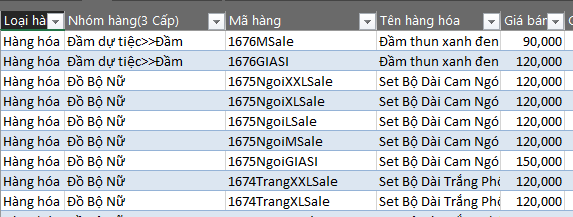
\includegraphics[width=0.9\textwidth]{imagev2/danhsachsanpham.PNG}
\caption{\label{fig:excelsample} Mẫu excel danh sách sản phẩm}
\end{figure}

Tập tin dữ liệu Excel nằm ở đường dẫn \url{csdlnc_util\\data\\DanhSachSanPham.xlsx}. Ta sẽ dùng các đoạn mã Python (thư mục csdlnc-util) để chuyển Excel thành Neo4j Cypher rồi chạy các cypher để nạp vào cơ sở dữ liệu. 

Yêu cầu các gói Python sau (có thể dùng câu lệnh pip install tên\_gói để cài đặt): 

\begin{itemize}
\item neo4j-driver
\item Unidecode 
\item openpyxl
\end{itemize}

Trước tiên, cần mỡ ex\_cypher\_file.py để thay đổi thông tin cơ sở dữ liệu. Tìm đoạn mã nguồn như Mã \ref{list:neo4jauth} và thay vào thông tin của Neo4j đã cài ở mục \ref{sec:installneo4jinstance}.

\begin{lstlisting}[language=python,caption={Thông tin Neo4j},label={list:neo4jauth}]
    uri = "bolt://188.166.233.199:7687"
    auth = ("tthien", "neo4jmeow")
\end{lstlisting}

Sau đó, chạy các dòng lệnh sau (Mã \ref{list:loadneo4jdata}) để nạp dữ liệu vào Neo4j.

\begin{lstlisting}[language=bash,caption={Cài Neo4j},label={list:loadneo4jdata}]
python import_product.py # chuyen Excel qua Cypher
python ex_cypher_file.py outcypher.txt # nap vao neo4j 
\end{lstlisting}

\subsection{Chatbot}
\subsubsection{Cài đặt tài khoản Bot trên Telegram}
Thực hiện các bước sau
\begin{itemize}
\item Tải ứng dụng Telegram vào điện thoại hoặc dùng bảng web \footnote{\url{https://web.telegram.org/}}
\item Tạo tài khoảng 
\item Liên hệ @BotFather \footnote{\url{https://t.me/botfather}} để tạo Bot và lấy API Token \footnote{API Token giống thế này: 681953844:AAF67DFPwTGuzHtPwZvGs1mjmLZ85IHTNmk}. 
\item Ghi lại tên bot và API Token 
\end{itemize}

\subsubsection{Chạy ứng dụng Chatbot}

Lần lượt chạy các đoạn Mã \ref{list:compiletelegrambot}, \ref{list:envtelegrambot}, \ref{list:runtelegrambot} để chạy bot. 

\begin{lstlisting}[language=bash,caption={Biên dịch mã nguồn},label={list:compiletelegrambot}]
gradle stage 
\end{lstlisting}

\begin{lstlisting}[language=bash,caption={Tạo các biến môi trường},label={list:envtelegrambot}]
export DEV_BOT_TOKEN=api_token
export DEV_BOT_NAME=ten_bot
export NEO4J_IP="localhost" 
export NEO4J_BOLT_PORT="7687"
export NEO4J_USERNAME="neo4j"
export NEO4J_PASSWORD=mat_khau_neo4j
\end{lstlisting}

\begin{lstlisting}[language=bash,caption={Chạy bot},label={list:runtelegrambot}]
java -jar build/libs/telegrambot-3.0-all.jar
\end{lstlisting}

\section{Đánh giá tốc độ} 

\subsection{Nạp dữ liệu}

Nap dữ liệu ban đầu, có tất cả 7689 câu truy vấn. Cypher được thực hiện trực tiếp trên máy có chứa Neo4j (driver kết nối vào localhost) hoàn thành trung bình trong 28 giây. 


\subsection{Sử lý yêu cầu từ người dùng}

Các câu sẽ dùng để thử 

\begin{itemize}
\item áo sơ mi
\item /re\_nhat áo sơ mi
\item /tim\_re\_hon 200000
\item /khoang\_gia 200000 300000
\item /tim\_loai áo
\item /liet\_ke\_loai
\item /cung\_loai 816f
\end{itemize}

Thời gian được tính từ lúc bot bắt đầu xử lý câu truy vấn đến khi bot ra được chuỗi string để sẵn sàng trả về cho người dùng (chuỗi -> cypher ->kết quả -> chuỗi trả về), đơn vị milisecond. Không tính thời gian tương tác với nền tảng Telegram (không bao gồm thời gian gởi và nhận dữ liệu đến Telegram). 

\subsubsection{Máy laptop cá nhân}
Máy cá nhân, Telegrambot và Neo4j nằm trên cùng 1 máy 

\begin{center}
 \begin{tabular}{||c c c c||} 
 \hline
Câu & Lần 1 & Lần 2 & Lần 3 \\ [0.5ex] 
 \hline
 \hline
áo sơ mi  & 62 & 12 & 12 \\ 
 \hline
/re\_nhat áo sơ mi & 16 & 32 & 15 \\
 \hline
 /tim\_re\_hon 200000 & 64 & 19 & 24 \\
 \hline
 /tim\_khoang\_gia 200000 300000 & 15 & 10 & 48 \\
 \hline
 /tim\_loai áo & 8 & 8 & 36 \\
 \hline
/liet\_ke\_loai & 20 & 8 & 16 \\
 \hline
  /cung\_loai 816f & 124 & 8  & 9 \\ [1ex] 
 \hline
\end{tabular}
\end{center}


\subsubsection{VPS}
Neo4j và Telegrambot nằm ở 2 VPS khác nhau, nhưng cùng nhà cung cấp dịch vụ Digital Ocean \footnote{\url{https://digitalocean.com}}. 

\begin{center}
 \begin{tabular}{||c c c c||} 
 \hline
Câu & Lần 1 & Lần 2 & Lần 3 \\ [0.5ex] 
 \hline
 \hline
áo sơ mi  & 184 & 17 & 19 \\ 
 \hline
/re\_nhat áo sơ mi & 84 & 25 & 10 \\
 \hline
 /tim\_re\_hon 200000 & 27 & 16 & 13 \\
 \hline
 /tim\_khoang\_gia 200000 300000 & 34 & 10 & 23 \\
 \hline
 /tim\_loai áo & 45 & 14 & 7 \\
 \hline
/liet\_ke\_loai & 8  & 6 & 4 \\
 \hline
  /cung\_loai 816f & 18 & 6  & 9 \\ [1ex] 
 \hline
\end{tabular}
\end{center}

\bibliographystyle{IEEEtran}
\bibliography{bib}

%%%%%%%%%%%%%%%%%%%%%%%%%%%%%%%%%%%%%%%%%%%%%%%%%%%%
% Comments can be added to the margins of the document using the \todo{Here's a comment in the margin!} todo command, as shown in the example on the right. You can also add inline comments too:

% \todo[inline, color=green!40]{This is an inline comment.}



% \subsection{Tables and Figures}

% Use the table and tabular commands for basic tables --- see Table~\ref{tab:widgets}, for example. You can upload a figure (JPEG, PNG or PDF) using the files menu. To include it in your document, use the includegraphics command as in the code for Figure~\ref{fig:frog} below.

% % % Commands to include a figure:
% % \begin{figure}
% % \centering
% % 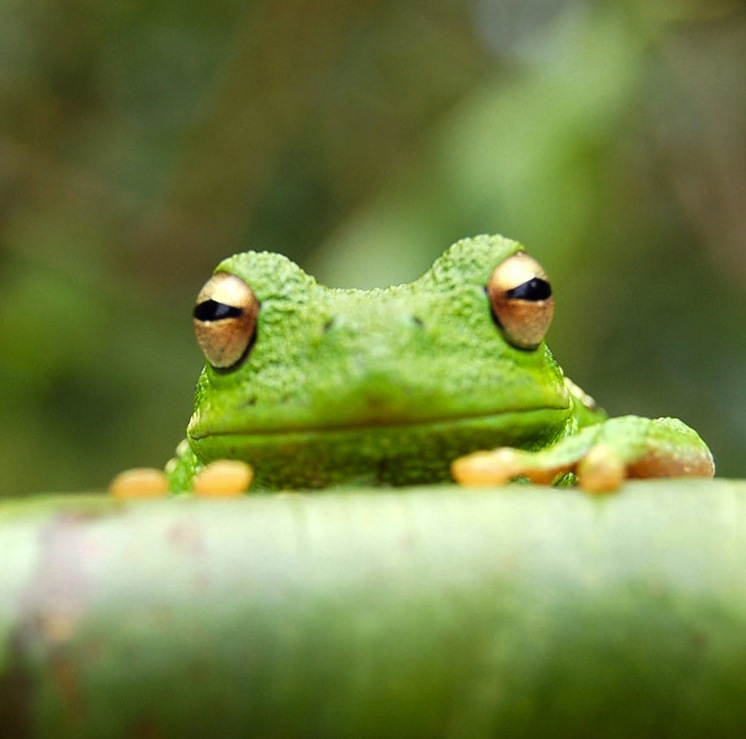
\includegraphics[width=0.5\textwidth]{frog.jpg}
% % \caption{\label{fig:frog}This is a figure caption.}
% % \end{figure}

% % \begin{table}
% % \centering
% % \begin{tabular}{l|r}
% % Item & Quantity \\\hline
% % Widgets & 42 \\
% % Gadgets & 13
% % \end{tabular}
% % \caption{\label{tab:widgets}An example table.}
% % \end{table}

% \subsection{Mathematics}

% \LaTeX{} is great at typesetting mathematics. Let $X_1, X_2, \ldots, X_n$ be a sequence of independent and identically distributed random variables with $\text{E}[X_i] = \mu$ and $\text{Var}[X_i] = \sigma^2 < \infty$, and let
% $$S_n = \frac{X_1 + X_2 + \cdots + X_n}{n}
%       = \frac{1}{n}\sum_{i}^{n} X_i$$
% denote their mean. Then as $n$ approaches infinity, the random variables $\sqrt{n}(S_n - \mu)$ converge in distribution to a normal $\mathcal{N}(0, \sigma^2)$.

% \subsection{Lists}

% You can make lists with automatic numbering \dots

% \begin{enumerate}
% \item Like this,
% \item and like this.
% \end{enumerate}
% \dots or bullet points \dots
% \begin{itemize}
% \item Like this,
% \item and like this.
% \end{itemize}

% We hope you find write\LaTeX\ useful, and please let us know if you have any feedback using the help menu above.

\end{document}